\documentclass[12pt,a4paper,oneside,oldfontcommands]{memoir}
\usepackage[utf8]{inputenc}
\usepackage[T1]{fontenc}
\usepackage{microtype}
\usepackage[dvips]{graphicx}
\usepackage{xcolor}
\usepackage{times}
\usepackage[super]{nth}
\usepackage{float}
\usepackage{subcaption}
\usepackage{multirow}
\usepackage[dvips]{graphicx}
\usepackage[
breaklinks=true,colorlinks=true,
%linkcolor=blue,urlcolor=blue,citecolor=blue,% PDF VIEW
linkcolor=black,urlcolor=black,citecolor=blue,% PRINT
bookmarks=true,bookmarksopenlevel=2]{hyperref}

\documentclass{article}
\usepackage[utf8]{inputenc}
 
\usepackage{listings}
\usepackage{color}
 
\definecolor{codegreen}{rgb}{0,0.6,0}
\definecolor{codegray}{rgb}{0.5,0.5,0.5}
\definecolor{codepurple}{rgb}{0.58,0,0.82}
\definecolor{backcolour}{rgb}{0.95,0.95,0.92}

\lstdefinestyle{mystyle}{
    backgroundcolor=\color{backcolour},   
    commentstyle=\color{codegreen},
    keywordstyle=\color{magenta},
    numberstyle=\tiny\color{codegray},
    stringstyle=\color{codepurple},
    basicstyle=\footnotesize,
    breakatwhitespace=false,         
    breaklines=true,                 
    captionpos=b,                    
    keepspaces=true,                 
    numbers=left,                    
    numbersep=5pt,                  
    showspaces=false,                
    showstringspaces=false,
    showtabs=false,                  
    tabsize=2
}

\lstset{style=mystyle}


\usepackage{geometry}
% PDF VIEW
%\geometry{total={210mm,297mm},
%left=25mm,right=25mm,%
%bindingoffset=0mm, top=25mm,bottom=25mm}
% PRINT
\geometry{total={210mm,297mm},
left=40mm,right=40mm,
bindingoffset=10mm, top=25mm,bottom=25mm}
\OnehalfSpacing
%\linespread{1.3}

%%% CHAPTER'S STYLE
\chapterstyle{bianchi}
%\chapterstyle{ger}
% \chapterstyle{madsen}
% \chapterstyle{ell}
%%% STYLE OF SECTIONS, SUBSECTIONS, AND SUBSUBSECTIONS
\setsecheadstyle{\Large\bfseries\sffamily\raggedright}
\setsubsecheadstyle{\large\bfseries\sffamily\raggedright}
\setsubsubsecheadstyle{\bfseries\sffamily\raggedright}


%%% STYLE OF PAGES NUMBERING
%\pagestyle{companion}\nouppercaseheads 
\pagestyle{headings}
%\pagestyle{Ruled}
%\pagestyle{plain}
\makepagestyle{plain}
\makeevenfoot{plain}{\thepage}{}{}
\makeoddfoot{plain}{}{}{\thepage}
\makeevenhead{plain}{}{}{}
\makeoddhead{plain}{}{}{}


\maxsecnumdepth{subsubsection} % chapters, sections, and subsections are numbered
\maxtocdepth{subsubsection} % chapters, sections, and subsections are in the Table of Contents

% \renewcommand{\baselinestretch}{2.0}

%%%---%%%---%%%---%%%---%%%---%%%---%%%---%%%---%%%---%%%---%%%---%%%---%%%

\begin{document}

%%%---%%%---%%%---%%%---%%%---%%%---%%%---%%%---%%%---%%%---%%%---%%%---%%%
%   TITLE PAGE
%
%   due to variety of title page schemes it is probably better to make titlepage manually
%
%%%---%%%---%%%---%%%---%%%---%%%---%%%---%%%---%%%---%%%---%%%---%%%---%%%
\thispagestyle{empty}

\begin{page}

\newcommand{\HRule}{\rule{\linewidth}{0.5mm}} % Defines a new command for the horizontal lines, change thickness here

\center % Center everything on the page
 
%----------------------------------------------------------------------------------------
%	HEADING SECTIONS
%----------------------------------------------------------------------------------------

\textsc{\LARGE University College Cork}\\[1.5cm] % Name of your university/college
\textsc{\Large BSc Computer Science}\\[0.5cm] % Major heading such as course name
\textsc{\large Final Year Project}\\[0.5cm] % Minor heading such as course title

%----------------------------------------------------------------------------------------
%	TITLE SECTION
%----------------------------------------------------------------------------------------

\HRule \\[0.4cm]
{ \huge \bfseries A Deep Learning Regression Model to Predict Galaxy Types Using The Galaxy Zoo GZ2 Data Set
}\\[0.4cm] % Title of your document
\HRule \\[1cm]
 
%----------------------------------------------------------------------------------------
%	AUTHOR SECTION
%----------------------------------------------------------------------------------------

\begin{minipage}{0.4\textwidth}
\begin{flushleft} \large
\emph{Author:}\\
Hassan \textsc{Baker} % Your name
\end{flushleft}
\end{minipage}
~
\begin{minipage}{0.4\textwidth}
\begin{flushright} \large
\emph{Supervisor:} \\
Prof. Gregory \textsc{Provan} % Supervisor's Name
\end{flushright}
\end{minipage}\\[1cm]

% If you don't want a supervisor, uncomment the two lines below and remove the section above
%\Large \emph{Author:}\\
%John \textsc{Smith}\\[3cm] % Your name

%----------------------------------------------------------------------------------------
%	DATE SECTION
%----------------------------------------------------------------------------------------

{\large \today}\\[2cm] % Date, change the \today to a set date if you want to be precise

%----------------------------------------------------------------------------------------
%	LOGO SECTION
%----------------------------------------------------------------------------------------

\includegraphics[width=4cm]{images/ucc.jpeg}
%----------------------------------------------------------------------------------------

\vfill % Fill the rest of the page with white space

\end{page}


\cleardoublepage
%%%---%%%---%%%---%%%---%%%---%%%---%%%---%%%---%%%---%%%---%%%---%%%---%%%
%%%---%%%---%%%---%%%---%%%---%%%---%%%---%%%---%%%---%%%---%%%---%%%---%%%

\begin{Abstract}
\thispagestyle{plain}
\addcontentsline{toc}{chapter}{Abstract}

\chapter*{Abstract}

\Large
 \begin{center}
A Deep Learning Regression Model to Predict Galaxy Types Using The Galaxy Zoo GZ2 Data Set\\ 

\hspace{10pt}

% Author names and affiliations
\large
Hassan Baker

\hspace{10pt}

\small  

\end{center}

\hspace{10pt}

\normalsize
\noindent

This project studies various aspects of deep learning, by using empirical comparisons. This study uses the Kaggle Galaxy Zoo Challenge \textit{GZ2} data set, containing images of galaxies, and probability distribution solutions. We carry out an experiment to find the optimal learning optimization algorithm, which involves a study of three algorithms. Furthermore, we find the optimal learning rate that corresponds to the chosen algorithm by carrying out a hyper-parameter search. This project studies the effects of using different activation functions in a deep learning model so as to select the most effective combination to lower error. We experiment with varying numbers of convolutional layers to assess the effect this has on the network. These studies are accomplished by building various deep convolutional neural networks that predict solutions on test set using TensorFlow. Through the various networks developed in this project, we overcome under-fitting by increasing the sizes of the networks, and tackle over-fitting by using dropout regularization and augmenting the data so as to produce more features. 

\end{Abstract}


\clearpage


\begin{Declaration Of OriginalityOrginality}
\thispagestyle{plain}
\addcontentsline{toc}{chapter}{Declaration Of Originality}

\chapter*{Declaration Of Originality}
\textbf{Declaration of Originality}

In signing this declaration, you are conforming, in writing, that the submitted work is entirely your own original work, except where clearly attributed otherwise, and that it has not been submitted partly or wholly for any other educational award.

I hereby declare that:
\begin{itemize}
\item this is all my own work, unless clearly indicated otherwise, with full and proper accreditation;
\item with respect to my own work: none of it has been submitted at any educational institution contributing in any way to an educational award;
\item with respect to another's work: all text, diagrams, code, or ideas, whether verbatim, paraphrased or otherwise modified or adapted, have been duly attributed to the source in a scholarly manner, whether from books, papers, lecture notes or any other student's work, whether published or unpublished, electronically or in print.
\end{itemize}
Signed:. . . . . . . . . . . . . . . . . . . . . . . . . . . . . . . . . . . . . . \\
Date: . . . . . . . . . . . . . . . . . . . . . . . . . . . . . . . . . . . . . . .

\end{Declaration Of Originality}

\clearpage


\begin{Acknowledgements}
\thispagestyle{plain}
\addcontentsline{toc}{chapter}{Acknowledgements}
\chapter*{Acknowledgements}

\end{Acknowledgements}

The work carried out in this project is dedicated to my parents, Nazar Baker, and Lamyaa Ridha, who have both, from an early stage, instilled a high level of appreciation and value for education onto myself, and my siblings. For that I am very thankful. 

I am especially thankful to Prof. Gregory Provan for all his highly insightful and helpful advice throughout the year, and for giving me this opportunity to take on a challenge in computer science that is very much new to myself. It is an understatement to say that I have a serious appreciation for this field now, and a majority of it comes from the guidance of Prof. Gregory Provan.

I am extremely indebted to David O'Byrne and the entire UCC computer science department's systems administration staff for giving me access to the GPU work station, and for David's immediate help throughout the year, anytime an issue came up. I can't stress how much I appreciate this as most of this project would not be possible without David's efforts.

I would also like to give great thanks to Prof. Derek G. Bridge for being an excellent lecturer, who's AI modules really helped clear many AI concepts in a very understandable way that is far better than resources that I have found.

I would like to give thanks to my friends and colleagues in my class and in Netsoc who have been an absolute treasure to be around. In many ways seeing how they work and all of the cool things they have done has been inspirational for me to continue challenging myself in the field of computer science. 

\clearpage


\tableofcontents*{}
\listoffigures


\clearpage

%%%---%%%---%%%---%%%---%%%---%%%---%%%---%%%---%%%---%%%---%%%---%%%---%%%
%%%---%%%---%%%---%%%---%%%---%%%---%%%---%%%---%%%---%%%---%%%---%%%---%%%

\def \learning_rate {\(4\times10^{-4}\) }


\chapter{Introduction}

\section{Galaxy Zoo}
Galaxy Zoo is one of the largest citizen science projects in the world. The project collects images of galaxies and invites the public to classify the images into set classes. The classification process is done by giving the citizens a set of questions to answer regarding the morphology of the galaxies in the images.  The public's assessment of the data is later aggregated and cleaned. The project managed to get more than 50 million classifications in its first year using images of galaxies taken from the Sloan Digital Sky Survey (SDSS). 

Galaxy Zoo 2 (GZ2) refers to the second phase of the project. The images in the \textit{GZ2} data set compromise of the brightest 25\% from the SDSS~\cite{Willett}. This dataset contains more than 300,000 images. The public was asked to classify the galaxies in the images into 11 classes, which contain sub classes. This accumulates to 37 possible classes altogether. The galaxies were classified by the public’s answering of questions like “Is the galaxy smooth and rounded, with no sign of a disk?” These questions form a decision tree of 37 possibilities, which are the labels of the dataset. 

    \begin{figure}[ht]
    \center
      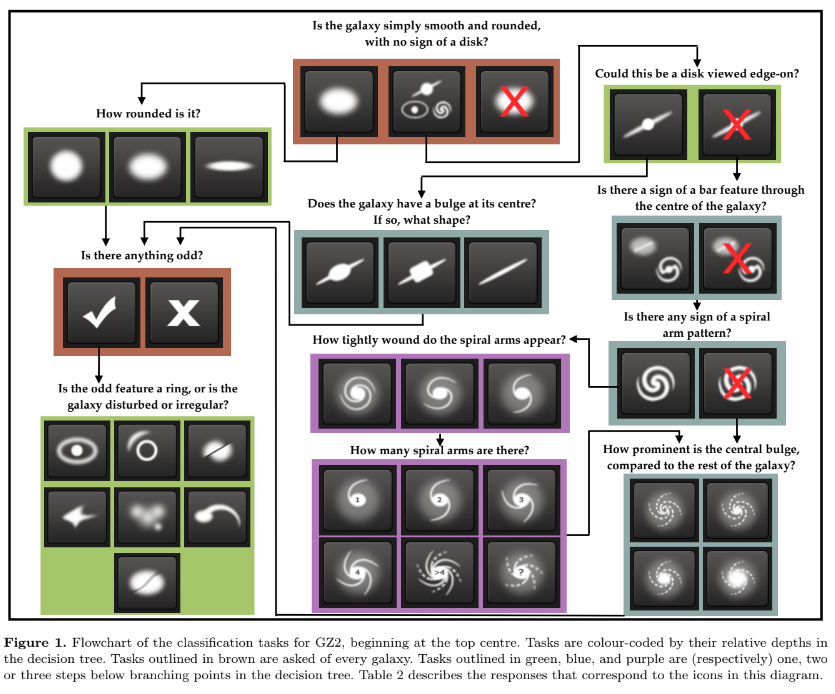
\includegraphics[width=\linewidth]{images/gz-2-decision-tree.png}
      \caption{Decision tree of galaxy labels in the GZ2 data set taken from Willett et al~\cite{Willett}.}
      \label{fig:GZ2-Decision-Tree}
    \end{figure}

\section{The Galaxy Challenge}

The Galaxy Zoo Galaxy Challenge was launched on the \nth{20} of December 2013 and hosted on Kaggle. The competition provided the set of \textit{GZ2} data. A set of probability distributions relating to what class the public judges each image to belong to is also given as a CSV files. The objective of the competition is to reproduce a CSV file of probability distributions for a test set, that reflects the public's assessment of these images. The majority of the solutions produced for this competition involved machine learning, and a majority of that majority relied heavily on convolutional neural networks.

Given the large set of image data, convolutional neural networks are an obvious choice as their use is proven to be highly effective in image recognition and analysis. However, convolutional neural network solutions, like many machine learning solutions, contain a level of complexity that originate from just how varying the model can be. One can refine at each step of the process to yield better accuracy or lower error, but in many ways, one can also over refine.

The competition had a total of \(326\) entrants, with most of the entrants achieving a private error in the range of \(0.2 < x < 0.1\). Furthermore, the \nth{50} ranking solution achieved a private test error of \(0.10146\), which starts the silver ranking of the leaderboard, with the top three solutions getting private scores of \(0.07491\), \(0.07752\), and \(0.07869\). In this project we will study the winning solution, the \nth{3} ranking solution, and a solution which ranked \nth{81} so as to accurately assess the networks developed. 

\section{Goals} \label{goals}

The main goal of this project is to develop a robust convolutional neural network that can produce a solution file for the test set with a low level of error, using Root Mean Squared Error (RMSE) for error estimation. We will aim to get a test error that would rank in the top 50 of the Kaggle competition. As a tangential goal, the student has undertaken this project to further their knowledge in deep learning methods and principles in a practical sense.


This model will be built incrementally by creating an initial model, and using it to study some key components of deep learning methods and architecture. Taking the results of these studies, the model will be improved to produce solutions with lower error. As the data is from a Kaggle competition from four years ago, there are already solutions available on the internet. The solutions examined in this study are Team 6789~\cite{Nguyen}, Fang-Chieh Chou~\cite{Fang}, and most notably Sander Dieleman~\cite{Sanders-GZ}. Hence this project focuses on studying some of the methods used in those solutions, as well as alternatives put forward by the student.The key areas of study in this project will focus on data preparation and processing, deep learning optimization algorithms, activation function comparisons, and hyper-parameter searching.

\subsection{Data Processing Study}

So as to get a better understanding of the data, this project aims to carry out an analytically study of the data. The results of the analysis will be used to better determine the architecture of the networks developed in this project, and how best to process the data. 

\subsection{Optimizer Comparison}
This project will aim to validate what the most fitting learning optimization algorithm to use, comparing Stochastic Gradient Descent (SGD), SGD with Nesterov Momentum, and Adam Optimization. This will be done simultaneously along with a learning rate search so as to find an optimal configuration. 

\subsection{Activation Function Comparison}
One of the goals if this project involves studying three different activation functions; sigmoid, ReLu, and maxout. The experiments will involve comparing these activation functions in different layers of the network and analyzing their effect. Specifically, we will study the effects of ReLu activation and sigmoid activation in the final layer of the network. Additionally, we will study the effects of using ReLu layers in the dense layers of a network compared to maxout layers, as described by Goodfellow et al~\cite{maxout}.

\subsection{Expected Problems \& Methods To Overcoming Them}
It is expected that many of the networks developed in this project will either under-fit or over-fit. Moreover, if a network is under-fitting, we will also increase the complexity of the network by increasing the size of the layers in a network, so it can fit more of the data.

In the case where network is over-fitting, we will implement dropout regularization to reduce this. Furthermore, we will look into decreasing the size of layers in the network.

\subsection{A Study Of The Winning Solution} \label{winning-sol}

We will aim to re-develop the network described by Sander Dieleman ~\citep{Sanders-GZ} in TensorFlow, as it Dieleman developed his solution using Theano. This project aims to dissect the effectiveness of this model by analyzing it and comparing it to the other models produced in this project.

\section{Achievements}

This project is largely successful in achieving the aims and goals highlighted. In total, we carried out three experiments, where the results and conclusions are used to improve the networks developed in this project. From these experiments we find the optimal learning algorithm andlearning rate combination is the Adam optimization algorithm at a learning rate of \learning_rate . Furthermore, we empirically find that a Relu rectifier is far superior to a sigmoid rectifier in the final layer of a network for this data set. Throughout this project we experience networks that under-fit and networks that over-fit, and successfully tackle both cases. Moreover, we experiment with the effects of changing the amount of convolutional layers used and the effects this has on the prediction error. We find that the difference of using three convolutional layers, to four convolutional layers, or five convolutional layers, is in fact negligible. In total, four different convolutional neural networks were built, two of which achieved error values that would rank in the top 50 of the Kaggle leaderboard, with the highest achieving a test error of \(0.09688\), which would rank it in the 38th spot in the Kaggle leaderboard.


\chapter{Methodology}

\section{Tools} \label{tools}

\subsection{Hardware}
The primary machine used in this project is one of the computer science department's GPU workstations, containing an Intel i7-6800K hexacore CPU and an Nvidia GTX 1080 GPU. However, so as to run multiple experiments at once, one of the UCC Netsoc (Networking and Technology Society) servers was used, leela.netsoc.co, which contains an Intel Xeon E5-2630.

\subsection{TensorFlow}
The main framework used is TensorFlow. TensorFlow offers a very intuitive method of for developing neural networks, with many examples available. It contains plenty of up to date features and a large support base. A key reason for the selection of TensorFlow is that it has a Python API as the student is very comfortable with Python. However, the most vital reason for the selection of TensorFlow is TensorBoard. It's highly difficult to debug neural networks. For the most part, the developer spends a majority of the time looking at graphs. The TensorBoard graphs are not only highly intuitive to code in TensorFlow, but also offer a lot more than alternatives like matplotlib. Moreover, TensorBoard simply offers a lot more, for a lot less work. For example, on the scalars view, there is a smoothing function which applies a linear filter to graphs so as to reduce noise as with gradient descent methods there tends to be a lot of rapid oscillations, which when plotted exactly can look like a mess. It is worth noting that throughout this project the reported error values used are after a smoothing factor of \(0.85\). This makes the data more concise and better reflects the models' performances.

The student has however experienced some negative aspects of working with TensorFlow. Although there are many examples and StackOverflow answers available, the documentation is quite lacking. The documentation tends to assume that you know what a certain method or object does and how it does it. There are cases where on the documentation page, rather than giving meaningful information, only a citation of the paper which the implementation replicates is described. Another example of bad documentation is the session storing feature, which allows the developer to save and restore a TensorFlow graph and session. There is simply too many ways of implementing this, and each offer different purposes with little documentation on what the purposes are. Luckily there are StackOverflow examples for this. Moreover, an even greater issue experience with TensorFlow is the inability to write custom activation functions, as there is currently no Python implementation for updating gradients throughout a TensorFlow graph. 

    \begin{figure}[ht]
    \center
      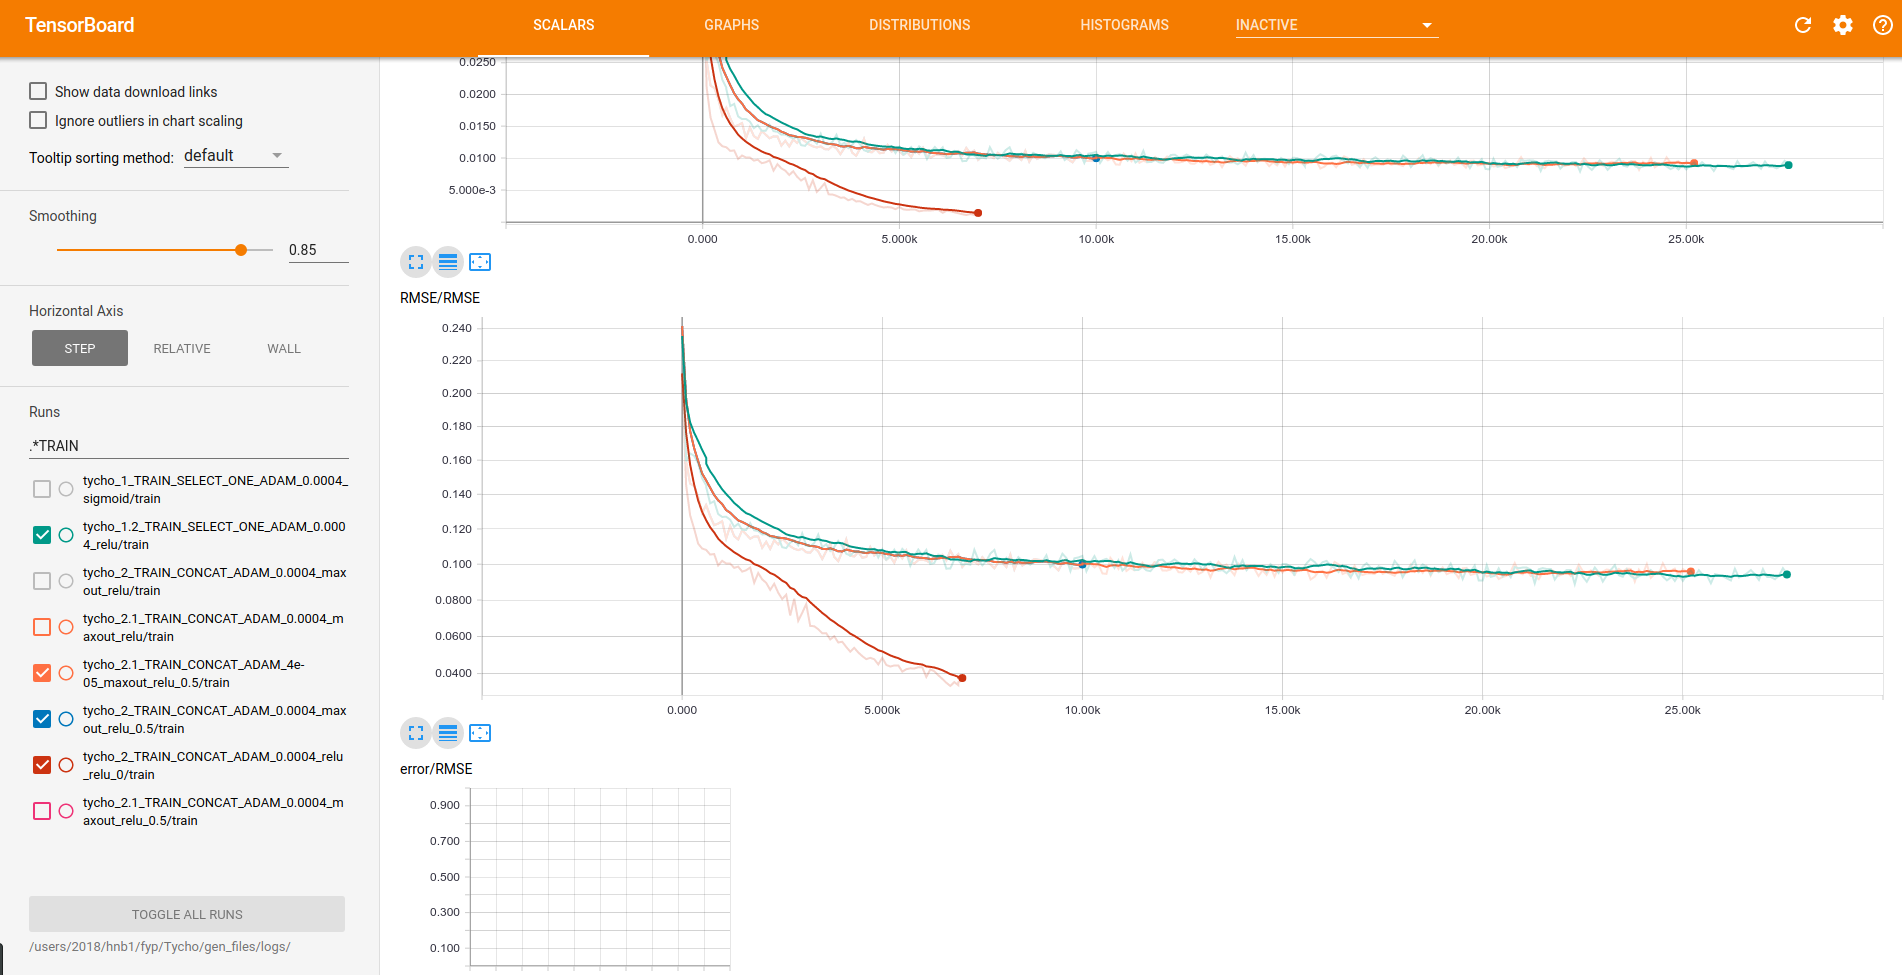
\includegraphics[width=\linewidth]{images/tensor_board.png}
      \caption{Screen-shot of TensorBoard scalars view}
      \label{fig:tb_sc}
    \end{figure}

Keras, an alternative to TensorFlow was considered at an early stage, however the student did not see any benefit to using it. It's a high level API that uses TensorFlow as the backend by default. This meant that the same performance would be available without the same amount of flexibility as TensorFlow provides. 
      

\subsection{IDE: Jupyter Notebook/PyCharm}
Initially Jupyter Notebook was used to develop the codebase as it offers a great documentation feature, which is very handy for machine learning projects. However many issues started to arise as the codebase got more complex. For instance, when a cell in a Jupyter Notebook is run, it is automatically cached in main memory. This is not only inefficient when working with a large dataset, but also problematic when working with TensorFlow, as when there is multiple Jupyter Notebooks running, conflicts between different TensorFlow graphs arise which make debugging harder than need be. This resulted in a lot of kernel restarts. Moreover, it was found that Jupyter Notebook simply encouraged bad coding habits, as it's easier to get in the habit of writing small scripts in the cells of a Jupyter Notebook, rather than modularising a code base for reuse. Hence the student switched to using the PyCharm IDE, which does not contain any of these issues. 

\section{Development}

As mentioned in Chapter \ref{tools}, the TensorFlow framework is used for the development of the convolutional neural networks in this project. The student found this framework to be very different to develop in, when compared to other more standard frameworks or libraries. The main difference is that it uses some abstract concepts, such as tensors, placeholders, and graphs. This made for a very different development experience than say a web framework. This is because one has to actually develop most of the components in the TensorFlow graph before being able to test that it works. Although it does have it's benefits, it makes it difficult to get started and learn the framework through practical work, and as mentioned before the documentation is pretty lacking.

In an early development stage, the student attempted to make the code-base entirely modular by developing a small library on top of the TensorFlow library that would automate the building of a network. This was done by the development of a network builder class, which reads a Python dictionary that describes a neural network, and iteratively builds the layers and components described in the dictionary while connecting them in the process, to result in one network at the end. An example of how this Python dictionary configuration can be seen in the code snippet below, which describes the Tycho1 network from chapter \ref{tycho1-arch}.

\lstinputlisting[language=Python]{network_dict.py}


A data processing mini library was also developed to read image data into a class and match images to their corresponding labels from a CSV file. This class also batches the data for training as the data is too large to load entirely into main memory. The same image data class uses a custom data augmentation class which contains methods for augmenting the data. The data augmentation class contains some low level augmentation methods, and some high level ones that consist of a combination of the lower level methods. These augmentation methods are described in section \ref{aug-section}. Currently, many of the methods in the data augmentation class are hard coded to suit this data set, but can easily be generalized with a few modifications. 

The network builder class was to be used in conjunction with a model analyzer class which would be used for training, validation and training. The issue experienced with this development process is that the student did not have enough experience with the TensorFlow library, hence it made debugging the networks and refining the network builder very troublesome. Hence this type of development was abandoned, and replaced with a more conventional procedural approach whereby networks are coded into files and run individually as a script, rather than one object that reads different configurations. This new approach proved to produce less risk, as it is far easier to debug, and modify.

However, many of the classes and tools from early development went into the later stages of development with little change. The model analyzer class is used throughout this project to validate networks, however it is not used for training, as the training configurations used ended up being more complex than anticipated. Furthermore, the data processing classes worked very well, hence are used throughout the later stages of development. One of the key tools that was taken from the network builder class, is the network blocks file. This is a file that consists of abstracted neural network objects, such as functions that return network components such as weights, biases, whole layers, or in some cases combinations of layers.

\section{Evaluation}

So as to empirically ensure improvements, a methodology will be adhered to throughout this project. Initially the data will be analyzed and a suitable convolutional neural network will be designed to fit the data. We will repeat a process of validation, training, and assessment.

To ensure the the network designed works as it is intended to, the network will be put through a validation stage, whereby it is trained for a small amount of time, on 90\% of the training set, allowing the remaining 10\% to be used for validation. Throughout the validation stage, the training and validation errors and losses are taken. 

On successful validation, we will move to a testing stage, whereby the network will then be trained for a longer period on the entire training set. Throughout the training solution files will be produced to get the test error.

After this training period, the network will be analysed as the training error, test error, and the solutions produced should offer insight as to how to improve on the current network.

Given the insights gained from training, a new network will be then be created to better fit the data. The new network will be put through validation and testing. 

We will assess the performance of a network by generating a set of predictions on the test set in the form of a CSV solution file. These solution files will be generated throughout the training over a set number of intervals so as to better understand how the model progresses through training. We will submit these solutions as a late submission in the Kaggle Galaxy Zoo Challenge page to get a private and public test error. Note, the public score is assessed using the approximately 25\% of the test set set, and the private score is assessed using approximately 75\%. Hence we will use the private score as it will be more reflective of the model's performance and compare this result to the other scores in the private leaderboard. 

It's worth noting that since access to the training set's labels is not available, this report will mainly focus on the error values, rather than loss values. However, throughout development, loss had proven to be quite effective for ensuring that the models are behaving as expected.

\chapter{Convolutional Neural Networks}

\section{Neural Networks}
Neural Networks are constructed by layers that consist of parallel neurons (represented by figure \ref{fig:neuron}) which contain weights and biases. The data is inputted into the first layer. At each neuron, the input is multiplied by the weight, and a bias is added to the solution. The output of each neuron is then put through a non-linear function. This is so as to introduce non-linearity in the network, as most models can be represented by non-linear functions. Each output is then passed into the following layer, abiding by the connection scheme i.e. in a fully connected network, each neuron passes it's output to every other neuron in the following layer as shown in figure \ref{fig:fully_connected}. 

    \begin{figure}[ht]
    \center
      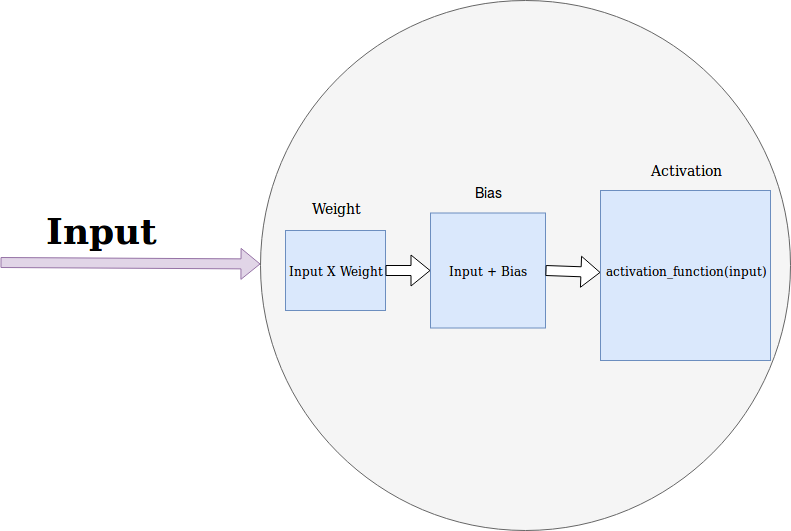
\includegraphics[width=12cm]{images/neuron.png}
      \caption{In neural networks, a neuron is an abstract object which multiplies an input with a weight, adds a bias, and carrys out a non-linear activation function.}
      \label{fig:neuron}
    \end{figure}
    
    \begin{figure}[ht]
    \center
      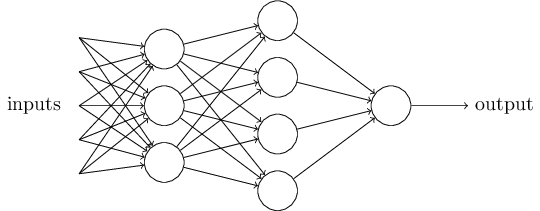
\includegraphics[width=\linewidth]{images/fully_connected.png}
      \caption{A fully connected network whereby all neurons in a \(layer_i\) are connected to all neurons in \(layer_i_+_1\). Image taken from http://neuralnetworksanddeeplearning.com/chap1.html}
      \label{fig:fully_connected}
    \end{figure}
    
The final layer in a neural network outputs the predictions, given an input. So as to give accurate predictions, the network is trained. Training involves the use of a labeled data set. By putting a set of training inputs through the network, and measuring the difference between what the network predicts and what the actual values it should predict are, one can calculate the loss. The loss is minimized throughout each training iteration using the back-propagation algorithm. Back-propagation updates the weight values in relation to partial derivatives of the gradient of the loss. This allows the model to predict better with repeated training ~\cite{rumelhart}. 

\section{Under-fitting \& Over-fitting}

Many of the networks developed in this project will be described as under-fitting or over-fitting. These terms relate to how the units (neurons) in the network fit the data. If one we're to abstract the neurons of a layer as a set of constants that biject a set of variable in a non-linear function, we are in a sense searching for the right values for these constants. However, when we come to the issue of how many constants (neurons) do we need. Having not enough constants means that we can only learn so much, so our network will learn a model that will best approximate the optimal model, but would never achieve it. Hence this is referred to as under-fitting. A sign that a network is under-fitting is when both the training error and the validation error are low. Furthermore, one can have too many constants. This results in the network needing to fit more of the data than need be as there are more constants in the model produced than the optimal model. Hence, the network will use some of the less important inputs to fit into the model, this usually means that the constants begin learning the parts of the input you don't want it to learn, i.e. the noise ~\cite{dgb}. This results in a very low training error as the network learns to recognize the noise in the data set, however, it also results in a relatively poor test error as it does not learn to generalize. So as to avoid under-fitting, it is recommended to increase the layer sizes in the network. However for over-fitting, it is recommended to either reducing the complexity of the network, getting more data, or generate new features using data augmentation, or use a regularization method, such as dropout, as described by Srivastava et al ~\cite{dropout}.

\section{Convolutional Neural Networks}

Convolutional neural networks methods are used widely for image recognition, sound recognition, natural language processing~\cite{Bhandare}, and a whole cohort of other applications.

Convolutional neural networks are currently one of the most popular machine learning techniques. They are powerful machine learning methods as they rely on breaking down the image into smaller convolutions and detects whether the learned patterns exist in these convolutions. The order and location of where these patterns occur is less important than in an ordinary feed-forward neural network, which is actually beneficial for particular tasks, such as image recognition.

Convolutional neural networks are more efficient to train and need less data than regular feed-forward networks, even though their theoretical maximum accuracy is not as good. This is because the convolutional layers that make them quicker to train than standard neural networks. These layers convolute the data into separate learning phases. An earlier layer would tend to take on the job of edge detection, and pass that information to the following layer. As you move through the layers, the learned filter should get more complex, until it eventually recognizes whole objects. This is because each individual layer can be seen as a separate network which is optimized, through training, to produce the easiest solution for the following layer to work with. 

This feature of convolutional neural networks allows for useful methods like transfer learning, whereby one can take the convolutional layers of one already trained network, attach a new fully connected layer to it, and train it to recognize something else entirely, far quicker than it would to train a whole new network.


\chapter{The Data}

The \textit{GZ2} dataset consists of 61,578 training images, 79,975 test images, a CSV file consisting of the 37 probability distributions for each example in the training set, as well as CSV files containing all one ones, all zeros and central pixel benchmarks for comparison when training. The test set solutions are not provided, instead one is required to generate a CSV file with their own solutions and submit them. Seeing as this is a large dataset, \textit{holdout} validation was used instead of \textit{k-fold}, as \textit{k-fold} would otherwise be far too time consuming. A validation set was created from 10\% of the training set. This 10\% portion was moved into its own directory and was not used for analysis or training. This allowed for \textit{holdout} validation throughout analysis and training.


    \begin{figure}[ht]
    \center
      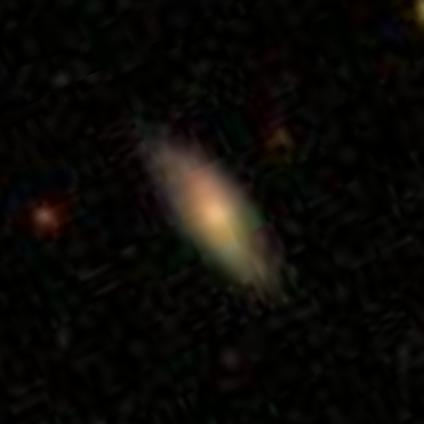
\includegraphics[width=7cm]{images/100023.jpg}
      \caption{An image of a galaxy from the GZ2 data set.}
      \label{fig:GZ2-1}
    \end{figure}
      

\subsection{Cropping} \label{Cropping}

The images in \textit{GZ2} are already centered and are \(424\times424\) in size. It does not seem feasible to fit every pixel of an example as a feature into the network as that would result in an input layer of shape \([424, 424, 3]\). This is far too big and would slow down learning greatly. The galaxies in the images are surrounded with black space. Sometimes these images contain some other stellar objects that have no apparent significance for the model. The black space and the stellar objects make for plenty of noise. Therefore it is only reasonable to uniformly crop these images so as to cut off a majority of the noise but still keep every galaxy intact. 

The winning solution, Sander Dieleman~\cite{Sanders-GZ} cropped the images to a standard size of \(207\times207\). However, there is no indication as to how the value \(207\times207\) was selected in this solution. 

To investigate this, using a Python script, all the images in the training set were analysed to validate this crop amount. The most important and active parts of the image are at the centre, accounting for most of the brightness in each image. Whereas the more dim areas are more likely to contain noise. Using brightness as a measure of activity, we can measure how much we have to crop each image to keep a selected threshold \(k\) of activity, \(k\) being the percentage of brightness in an image. Hence, each image’s colour channels are normalized to fit a the range \(0 < i < 1\), and are averaged into 1 channel (gray-scale).

Each individual image is then iteratively cropped towards the centre. In each iteration a 1 pixel wide perimeter was cropped out of the image. \(k'\), the percentage of brightness of an image was taken at each iteration. Once \(k'\) falls below \(k\), the amount of iterations carried out for that particular image are appended to a list \(Z\).

Once the whole training set is analysed, the mean of the values in \(Z\) is taken. Using trivial geometry, one can then determine the optimal crop amount for a mean of \(k\) brightness in the images. The mean value of \(z\), denoted by \(z\) amounts to how many pixels down the diagonal of the image to crop from. Given the value \(H\), the length of the diagonal from one corner of the original image to the opposite corner. This means that the length of the diagonal from one corner to the opposite corner of a cropped image, \(h\) is found using \(h = H - 2z\). Furthermore, seeing as the crop results in square dimensions, taking the dimension values as \((x, x)\), \(x\) can be found using Pythagoras. 

In this analysis, \(k\) was selected to be 90\%. This yielded a mean crop size of \(186\times186\), which is approximately \(20\times20\) smaller than the \(207\times207\) amount selected in Dieleman's solution~\cite{Sanders-GZ}, and \(14\times14\) smaller than the \(200\times200\) amount used by Team 6789~\cite{Nguyen}. Which leads to a conclusion that the crop amount in these solutions was either selected with good intuition, which is very possible, or else selected in a similar fashion with an extra ~10 pixels added in every direction for extra measure so as to make sure that outliers do not impact the results. To verify this, along with the mean crop amount, the maximum and minimum crop amounts for \(k=90\%\) were also taken. The maximum crop amount was \(398\times398\), and the minimum was a crop amount of \(0\times0\). It is easy to see how the minimum and maximum could skew this investigation by just looking at the image itself. The effect of outliers can be seen even clearer when plotting the crop amounts to a histogram (figure \ref{fig:crop_histogram}, which shows that there is a very large number of images effected by noise from extra stellar objects. These objects emit plenty of light which results in crop amounts of \(424\times424\), the exact size of the image.


\begin{figure}[H]
  \centering
  \begin{subfigure}[b]{0.4\linewidth}
    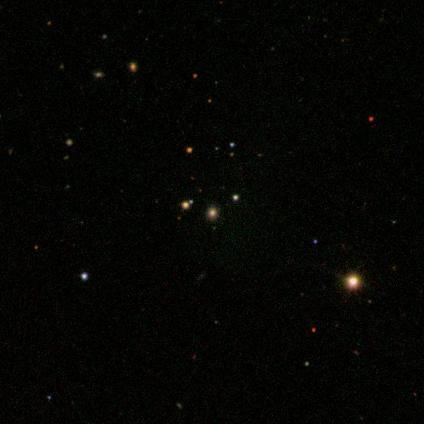
\includegraphics[width=\linewidth]{images/maximum-256411.jpg}
    \caption{The image requiring maximum crop, because the galaxy is very small and is easily confused with other stellar objects.}
  \end{subfigure}\hspace{1cm}
  \begin{subfigure}[b]{0.4\linewidth}
    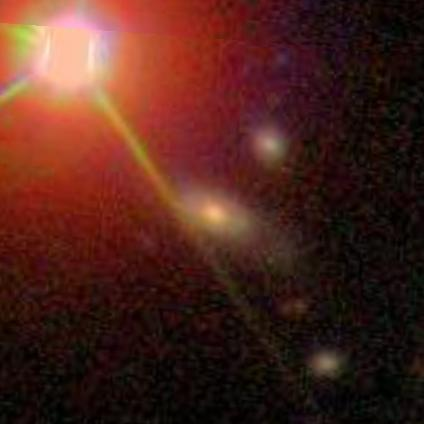
\includegraphics[width=\linewidth]{images/minimum-308196.jpg}
    \caption{The image that requires minimum crop due to the very bright stellar object is in the top right corner.}
  \end{subfigure}
  \caption{Outlier images found in GZ2}
  \label{fig:GZ2-2}
\end{figure}

\begin{figure}[ht]
    \center
      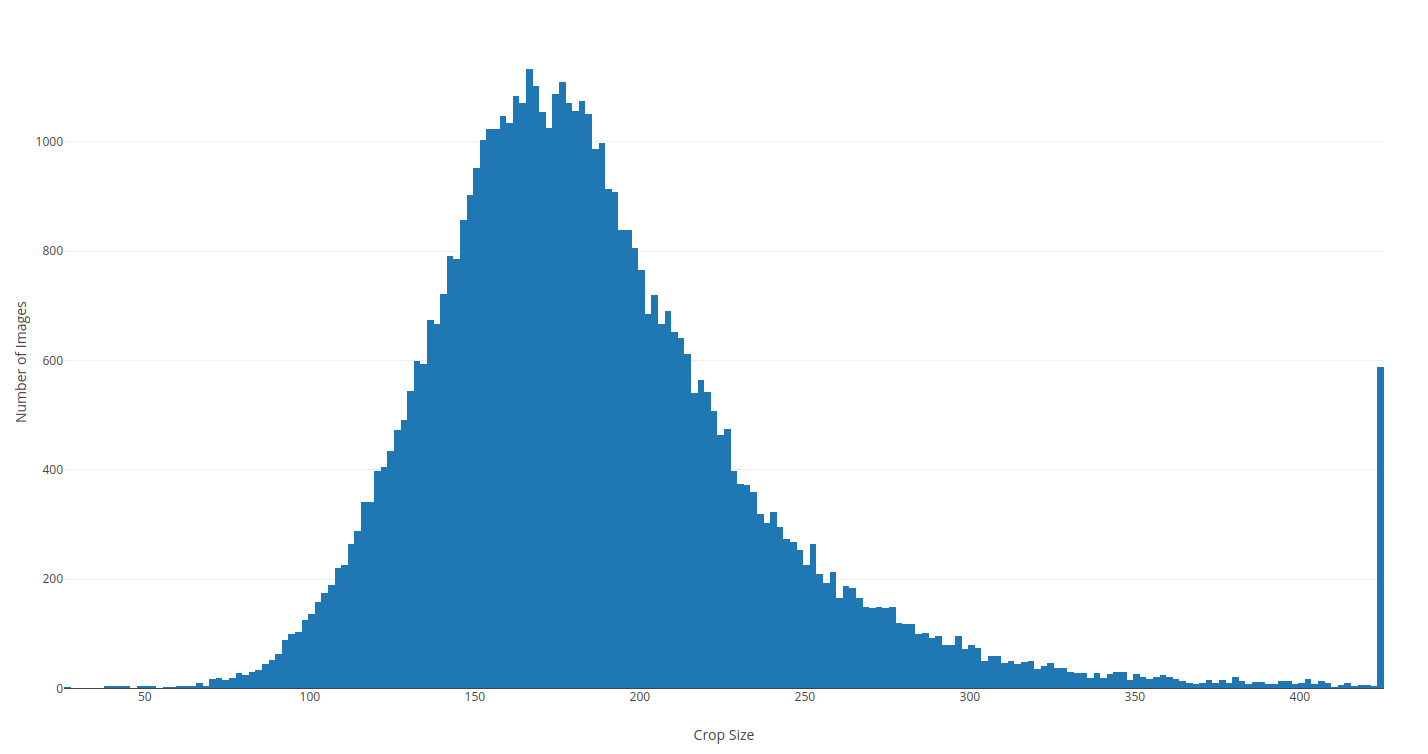
\includegraphics[width=\linewidth]{images/crop_analysis.png}
      \caption{A histogram of the crop amounts of each image in 90\% of the training set. It's very clear that outliers do effect the results, as there plenty of images with very high crop sizes, which is a result noise from extra stellar objects.}
      \label{fig:crop_histogram}
\end{figure}

So as to keep to account for outliers, and to stick to comparable measure, the crop amount that was selected in this study is \(207\times207\), the same used in Dieleman's solution~\cite{Sanders-GZ}.

\subsection{Down-scaling}

Cropping alone, still results in a very input large size as it would result in an input layer with 128,547 parameters, which will still stagnate the learning time, as all these parameters will have to be updated. Hence, the images were down-scaled by a factor of 1/3, as seen in Dieleman's solution~\cite{Sanders-GZ}. This results in the images taking the shape of \([69, 69, 3]\).

\subsection{Data Augmentation} \label{aug-section}

The images in the \textit{GZ2} data set contain exploitable variances. For instance, as they are images of galaxies, there is no up or down, or left or right. They are of uniform shapes, meaning that it is relatively easy to extract new features out of the given features. 

Inspired by the augmentation section in Dieleman's solution~\cite{Sanders-GZ}, a class for augmenting images was written. This class contains methods for cropping, down-scaling, rotation, and flipping. Using this class, one can can augment an image to extract 16 examples out of each individual image.

The augmentation process is thus. The \(207\times207\) crop is applied to each image, a 45 degree rotation of that same image, as well as a horizontal flip of the unaltered image, and the rotated one. This produces four images. This is illustrated in figure \ref{fig:sanders-aug-1}. 

\begin{figure}[H]
  \centering
    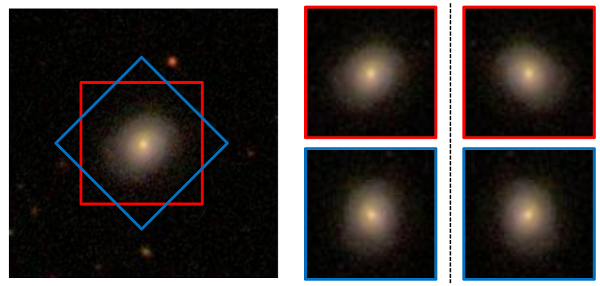
\includegraphics[width=\linewidth]{images/sanders-aug-1.png}
    \caption{Visualization of how 4 features are extracted from one image. Figure taken from Sander Dieleman's blog~\cite{Sanders-GZ}}
    \label{fig:sanders-aug-1}
\end{figure}

Furthermore, four crops of \(45\times45\) overlapping parts are taken from each corner of the images extracted, which produces 16 images in total. The 16 images are then rotated to ensure that all extracted images are oriented so that the galaxy is at the bottom right.


\begin{figure}[H]
  \centering
    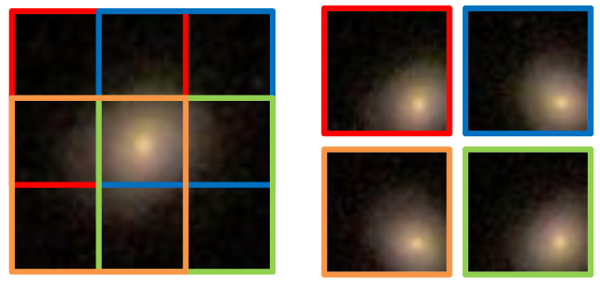
\includegraphics[width=\linewidth]{images/sanders-aug-2.png}
    \caption{Visualization of how the four overlapping parts are extracted from each images created in \ref{fig:sanders-aug-1}. Figure taken from Sander Dieleman's blog~\cite{Sanders-GZ}}
    \label{fig:sanders-aug-2}
\end{figure}

These extracted images overlap by design. This is so as to increase parameter sharing in the model. The bottom right of all extracted images contains the centre of the galaxy, however, the top right contains black space, or noise. Due to this augmentation, the values of the noisy sections are generally different in each extracted image, hence this process makes it more likely for a model to be more active with the bottom right sections.

\chapter{The Network: Tycho1}

The initial convolutional neural network, named Tycho1 is a modified version of the model described in Dieleman's blog ~\cite{Sanders-GZ}. It contains four convolutional layers, and three dense layers. Tycho one differs from Dieleman~\cite{Sanders-GZ} in the dense layers, and does not perform a concatenation on augmented image segments after they have passed the convolutional layers. This is because Tycho1 is designed to train faster, so as to validate the studies regarding learning optimization algorithms, learning rate searching, and activation function comparisons. 

\section{The Architecture} \label{tycho1-arch}

\begin{figure}[H]
  \centering
    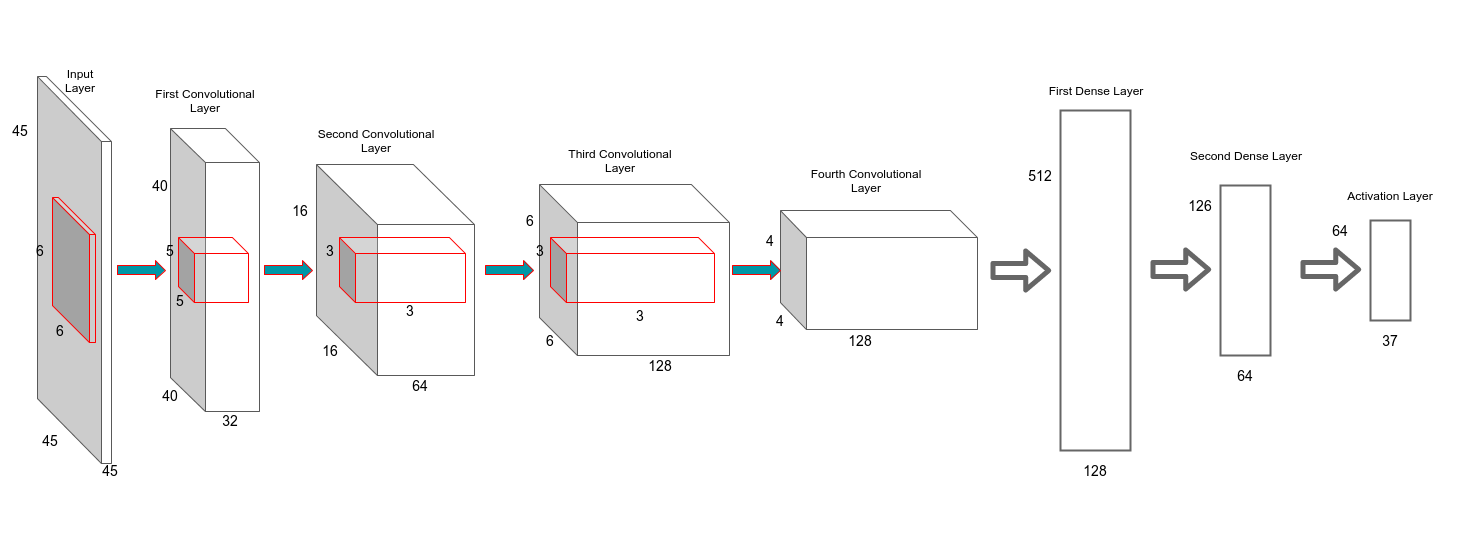
\includegraphics[width=\linewidth]{images/Tycho1.png}
    \caption{Diagram of the Tycho1 network}
    \label{fig:tycho1}
\end{figure}


The input layer takes inputs of shape \([BATCH\_SIZE, 45, 45, 3]\). The first element is the amount of images in a given batch, the second and third represent the size of each image, and the last element is the number of channels. This is then fed into the convolutional segment.

The network consists of four convolutional layers. The first convolutional layer contains a filter of size \(6\), and an output shape of \(32\). The second layer contains a filter of size \(5\) and an output shape of \(64\). The third and fourth both have a filter size of \(3\), and an output size of \(128\). The first, second, and fourth layers are followed by \(2\times2\) max-pooling layers. Once the data passes through the last convolutional layer, it is flattened into a shape of \([256, 512]\).

The flattened output then enters the dense layers. The weights in the first dense layer and the second dense layer are of shapes \([512, 128]\) and \([128, 64]\), respectively. 

All layers, bar the last contain a Rectified Linear Unit (ReLu) as the activation function.

\begin{equation}
    f(x)=max(x, 0)
    \label{eq:relu}
\end{equation}

\begin{figure}[H]
  \centering
    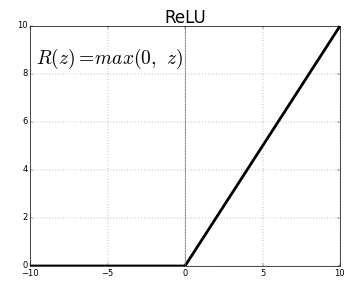
\includegraphics[width=7cm]{images/relu.png}
    \caption{Graph of ReLu activation. Taken from https://towardsdatascience.com/activation-functions-neural-networks-1cbd9f8d91d6}
    \label{fig:relu_graph}
\end{figure}

The ReLu activation function was chosen as it is extremely useful for object recognition ~\cite{ReLu}. A distinct feature of ReLu activation is that it has sparse activity allowing for mostly meaningful activations to be passed onto the next layer. This decreases training time, and makes activations far more efficient.

The weights in all layers, dense and convolutional, except the last, are initialized to be in a normal distribution of standard deviation \(0.01\), and a mean of \(0\). This restricts the weights to a range of \(-0.01 < W < 0.01\). 

The biases in all layers, including the last, are set to be a constant of \(0.1\). This was originally set to \(0.0\), but after some testing, \(0.0\) proved to be ineffective and resulted in dead units. Hence \(0.1\) is used instead.

The last layer is also a dense layer. This is of shape [BATCH\_SIZE, NUM\_LABELS].This shape corresponds to the amount of images to fed into the network, and the number of values/labels to predict. With this data, there are \(37\) labels.  The weights are initialized to be in a normal distribution of standard deviation \(0.001\), and a mean of \(0\). 

As described by Dieleman ~\cite{Sanders-GZ} and Fang-Chieh ~\cite{Fang}, a modified version of ReLu or Softmax, with a normalization segment was initially considered. However this is where TensorFlow has it's drawbacks, as there is no way to write custom activation functions using the TensorFlow Python API.

As an alternative, Sigmoid activation \ref{eq:sigmoid} is chosen for the last layer. This seems like the best fit as it squashes all values between a range of \(0 < y' < 1\).

\begin{equation}
    h(x) =  \frac{\mathrm{1} }{\mathrm{1} + e^-x }
    \label{eq:sigmoid}
\end{equation}

\begin{figure}[H]
  \centering
    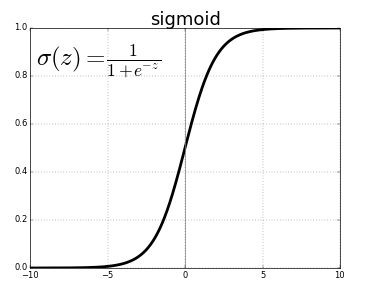
\includegraphics[width=7cm]{images/sigmoid.png}
    \caption{Graph of sigmoid activation. Taken from https://towardsdatascience.com/activation-functions-neural-networks-1cbd9f8d91d6}
    \label{fig:sigmoid_graph}
\end{figure}

The error evaluation function used for the Kaggle competition is Root Mean Squared Error (RMSE), hence, for measuring loss, Mean Squared Error (MSE) was used, so as to avoid using the same function for measuring loss and error.

\begin{equation}
     MSE = \frac{1}{n}\Sigma_{i=1}^{n}{({y_i -y'_i})^2}
\end{equation}

\begin{equation}
     RMSE = \sqrt{\frac{1}{n}\Sigma_{i=1}^{n}{({y_i -y'_i})^2}}
\end{equation}

Where \(n\) is the the batch size, or more generally, the number of predicted outputs. \(y\) is the the correct answers given a prediction, and \(y'\) is the predicted output.

\section{Missing Component}
There's a vital missing component in Tycho1 that has been purposely left out. This is the learning optimization algorithm. This will be studied further and decided on in chapter \ref{study1}

\section{Data Pre-processing} \label{tycho-data}

Just like most Kaggle competitions, the \textit{GZ2} dataset contains more examples in the test set than the training set. To accommodate for this, the image augmentation described in \ref{aug-section} is used. However, unlike Dieleman's model ~\cite{Sanders-GZ}, the resulting 16 images from the augmentation process we’re not concatenated. Instead, one random image from those 16 generated was selected. This serves to create more inputs to help the model generalize more towards the active parts of each image (bottom right, where the galaxies are), and reduce chances of over-fitting. 

\chapter{Study: Learning Optimizer Algorithms \& Hyper-Parameter Search} \label{study1}

A major key to deep learning is the learning optimization algorithm. The model described by Dieleman ~\cite{Sanders-GZ} details the usage of Stochastic Gradient Descent (SGD) of an initial learning rate of \(4\times10^{-2}\), and a Nesterov momentum of \(0.9\). 

However, there are alternatives to this algorithm. Most notably, SGD without Nesterov momentum and Adam optimization. A comparison of these algorithms was made on separate learning rates so as to empirically decide on the most suitable.

\section{Experiment Description}

The Tycho1 network was set up to take an input of a mini-batch of \(16\) images, that are augmented \(16\) times each, with one of the augmented image chosen at random. This model would train for \(2000\) epochs.

To compare the algorithms, the training was run in a loop to try out the different algorithms along with four different learning rates \(4\times10^{-2}\), \(4\times10^{-3}\), \(1\times10^{-4}\), and \(1\times10^{-4}\). Throughout these iterations, the loss and error values on both the training set and validation set is taken every 10 epochs. TensorBoard proved to be a vital tool for carrying out this comparison. It made it so that the loss and error values were stored and easily compared by overlaying them through the UI.

Each algorithm took roughly thirty five minutes to complete one iteration on one learning rate, so the whole comparison took about 7 hours to complete.

\section{Results}

\subsection{Stochastic Gradient Descent}

Stochastic Gradient Descent performed well on the first learning rate, \(4\times10^{-2}\), producing an RMSE of \(0.1702\) on the training set, and \(0.1735\) on the validation set, on the final epoch. However, when the learning rate was decreased, it performed very poorly, resulting in training and validation RMSE of approximately \(0.45\) for all other learning rates.

\subsection{Stochastic Gradient Descent With Nesterov Momentum}

SGD with Nesterov momentum proved even more effective on the \(4\times10^{-2}\) learning rate, producing a training and validation RMSE of \(0.1680\) and \(0.1611\) on the validation set on the final epoch. However, as the learning rate decreased, the performance decreased too. Interestingly though, the decrease was not as drastic as SGD without Nesterov momentum, as on the \(4\times10^{-3}\), it achieved a training and validation RMSE of \(0.17390\), and \(0.1708\) respectively. This algorithm did however result in error values of about \(0.45\) on the last two learning rates, just as the previous algorithm did.

\subsection{Adam} \label{Adam}

On the first learning rate, the Adam algorithm achieved considerably greater results than other algorithms, producing an RMSE of \(0.1705\) and \(0.1632\) on the training and validation sets respectively on the final epoch, with the learning rate of \(4\times10^{-2}\). This performance did however decrease on the second learning rate of \(4\times10^{-3}\), to being \(0.2418\) and \(0.2499\) for training and validation, respectively. Moreover, on the learning rate of \(4\times10^{-4}\). It did however decrease to a train RMSE of \(0.1517\) and a validation RMSE of \(0.1479\). For the learning rate of \(1\times10^{-4}\) it achieved an RMSE of \(0.1663\), and \(0.1671\) on the training and validation sets respectively. These results showed that the Adam algorithm was far more suitable and stable for this model. 

\subsection{Further Learning Rate Tests On The Adam Algorithm}

From the results of section \ref{Adam}, it looks apparent that lower learning rates perform better, with the exception of the first learning rate of \(4\times10^{-2}\). So in that vain, to smaller learning rates of \(4\times10^{-5}\) and \(4\times10^{-6}\) were tested with the same configuration as the tests above but produced lower RMSE values than it did with a learning rate of \(4\times10^{-4}\).

\begin{figure}[H]
    \centering
    \begin{tabular}{ |c|c|c|c|c| } 
    \hline
    Algorithm & Learning Rate & Training RMSE & Validation RMSE \\
    \hline
    \multirow{4}{4em}{SGD}
    & \(4\times10^{-2}\) & \(0.1702\) & \(0.1735\)\\ 
    & \(4\times10^{-3}\) & \(0.4383\) & \(0.4403\)\\ 
    & \(4\times10^{-4}\) & \(0.4518\) & \(0.4505\)\\ 
    & \(1\times10^{-4}\) & \(0.4552\) & \(0.4522\)\\
    \hline
    \multirow{4}{4em}{Nesterov}
    & \(4\times10^{-2}\) & \(0.1680\) & \(0.1611\)\\ 
    & \(4\times10^{-3}\) & \(0.1739\) & \(0.1708\)\\ 
    & \(4\times10^{-4}\) & \(0.4362\) & \(0.4365\)\\ 
    & \(1\times10^{-4}\) & \(0.4482\) & \(0.4485\)\\
    \hline
    \multirow{4}{4em}{Adam}
    & \(4\times10^{-2}\) & \(0.1705\) & \(0.1632\)\\ 
    & \(4\times10^{-3}\) & \(0.2418\) & \(0.2499\)\\ 
    & \(4\times10^{-4}\) & \(0.1517\) & \(0.1479\)\\ 
    & \(1\times10^{-4}\) & \(0.1663\) & \(0.1671\)\\
    & \(4\times10^{-5}\) & \(0.1649\) & \(0.1676\)\\ 
    & \(4\times10^{-6}\) & \(0.1676\) & \(0.1758\)\\
    \hline
    \end{tabular}
    \caption{The resultant RMSE's for each learning rate on each algorithm}
    \label{fig:learning_rates_table}
\end{figure}

\section{Conclusion} 
As the Adam algorithm performed the best on all learning rates, that will be the chosen algorithm for the models. This means that no further experiments will be done on learning rates, or learning rate schedules, as the Adam optimizer has it's own form of decay. Furthermore, by looking at the graphs on TensorBoard of all the tests carried out on the Adam algorithm, with a smoothing of \(0.85\), the learning rate of \(4\times10^{-4}\) seemed to be a marginally better choice than \(4\times10^{-2}\), even though it began to converge later, it ended with a lower RMSE. Furthermore, it also sloped further down than the learning rate of \(4\times10^{-2}\), indicating that it will perform even better if it was run further. Hence the chosen learning rate is \(4\times10^{-4}\). 

\chapter{Tycho1 - Evaluation} \label{tycho1} 

\section{Training Details}

A training script was written for the Tycho1 model using the Adam Optimizer, on a learning rate of \(4\times10^{-4}\) The script is set to train on a mini-batch of 256, using the full training set (including the data used in validation for chapter \ref{study1}), for 10,000 epochs. During the tests in chapter \ref{study1}, it was noticed that recording the logging summaries took a substantial amount of time, when compared to training, hence the recording interval is set to 100. This means that the TensorBoard log summary was taken every 100 epochs. A nice side effect of this is smoother graphs.

Taking away more data from the training set for validation does not seem viable here, as the training set itself is already smaller than the test set. Hence, the entire training set is used. Throughout the training, a CSV solution file for the test set is generated and tested on the Kaggle submission so as to ensure that the model is learning, and to better assess it's progress. The solution file is generated by a TEST\_INTERVAL parameter set in the code. 

Unfortunately there was an error in the code, that made it so test conditions were never satisfied. However the status of the model was saved every 100 intervals, allowing the training to be paused and for the script to be altered so as to meet these conditions and produce the test results. Hence we will the test results do not match the test interval. 

As the training surpassed \(10,000\), it becomes apparent that there is still room for improvement, and that training the model further could in fact keep improving the results.This can be seen in figure \ref{fig:tycho1-tb}. Hence, it was allowed to train for another day and a half. In total training took four days, including the time taken to generate the predictions on the test file, which on average took 45 minutes to generate. 

Furthermore, as the training started to produce results, it produced some very low values, but no hard \textit{zero's}. This was a known consequence of using Sigmoid activation in the final layer. However, the impact seemed greater as the training went on, as the more training is done the values that should be zero, tend closer to zero, but never get to zero. Hence we see a very drastic retardation in loss and error. So as to test this, the code regarding the custom activation layer from Dieleman ~\cite{Sanders-GZ} was adapted so as to normalize the prediction on the test set. This normalization was practiced when the training reached the \nth{12,000} epoch, and onward from there. 

\section{Results}

\begin{figure}[H]
  \centering
    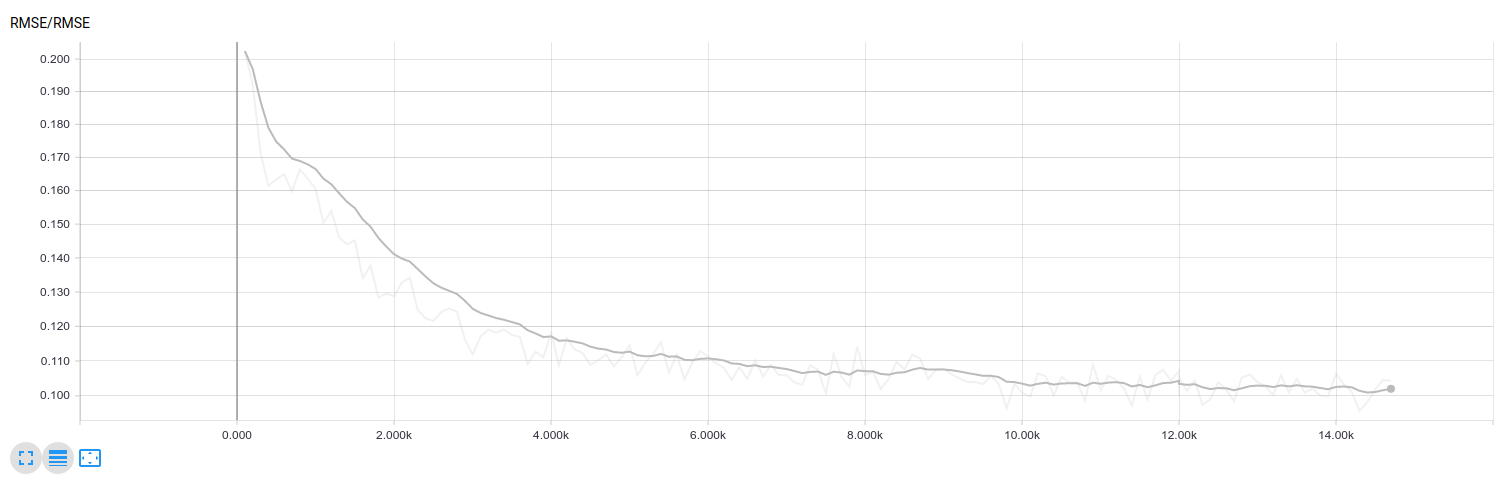
\includegraphics[width=\linewidth]{graphs/B/tycho_1_TRAIN_SELECT_ONE_ADAM_0004_sigmoid.png}
    \caption{TensorBoard graph of Tycho1 network training (with a smoothing of 0.85 applied)}
   \label{fig:tycho1-tb}
\end{figure}

\begin{figure}
\begin{center}
 \begin{tabular}{||c | c | c||} 
 \hline
 Epochs & Training Error & Test Error \\ [0.5ex] 
 \hline\hline
 27102 & 0.1252 & 0.12111\\ 
 \hline
 4001 & 0.1181 & 0.11452\\
 \hline
 6901 & 0.1060 & 0.10968\\
 \hline
 8203 & 0.1020 & 0.10636\\
 \hline
 9004 & 0.1077 & 0.10635\\ 
 \hline
 11005 & 0.1016 & 0.10446\\ 
 \hline
 12000 & 0.1072 & 0.10283\\ 
 \hline
 12000 - Normalized & 0.1072 & 0.10278\\
 \hline
 14700 & 0.1043 & 0.10239\\ 
 \hline
 14700 - Normalized & 0.1043 & 0.10220\\ [1ex] 
 \hline
\end{tabular}
\end{center}
\end{figure}

The final RMSE of 0.10220 would rank the Tycho1 model \nth{55} out of the 326 participants in both the private and public leaderboards of the Kaggle Galaxy Zoo competition. This puts it in the bronze ranking, and 5 spots away from a silver ranking. 

\begin{figure}[H]
  \centering
    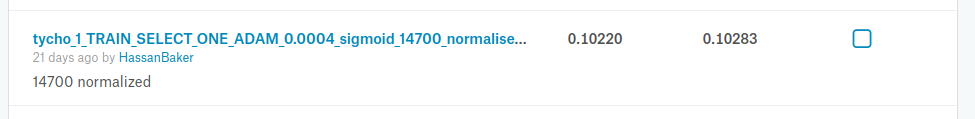
\includegraphics[width=\linewidth]{images/tycho1_result.png}
    \caption{Kaggle submission result of Tycho1 network after 14700 training epochs with a normalized solution)}
   \label{fig:tycho-1-solution}
\end{figure}

\section{Conclusion}

The Tycho1 network does seem to under-fit the data, however not very much, as it has successfully generated a model with what is empirically a good ranking by the competitions standards. However, some issues have come to light from this training.

Normalizing the output, does indeed improve the results, albeit slightly. This makes it apparent that a more suitable activation function is need in the final layer, as although one can normalize the output, the model cannot calculate the gradient for the normalized output on the training set. Hence, it cannot update variable values accordingly to these values. 

Although the Sigmoid activation function does produce decent results, it does hit a limit very quickly, which stagnates
learning greatly.

Allowing the network to run for another day or two would very likely get it in the silver ranking, however, this is not a very effective strategy, as the Tycho1 model does show some heavy signs of retardation when it it comes to loss, and error.

An important conclusion to note, is that the training errors and test errors are reasonably close to each other, indicating that the assumption of the validation set being to small is correct. This means that we can expect validation loss and error to be lower than training loss and error throughout.

\chapter{Tycho1.2 - Evaluation} \label{tycho1.2}

So as to improve on the Tycho1 network, ReLu activation is considered for the final layer of the Tycho1.2 network. The hypothesis here is that although ReLu does not restrict the output to a range of \(0 < x < 1\), it shouldn't be an issue as the input is already normalized to that range, and all the variables in the network (weights and biases) are bound to that range as well. Moreover, a required feature of ReLu is it's ability to detect hard zeros, which the model contains plenty of.

\section{Validation}

So as to validate this hypothesis, an experiment on the Tycho1.2 network is run with the Adam optimizer at a learning rate of \(4\times10^{-4}\) on a mini-batch of 16 for 2000 epochs. This is the same configuration used in the validation of of Tycho1 in section \ref{study1}. Hence we compare the results of the Tycho1.2 validation to the results of Tycho1 with the same learning optimization algorithm and learning rate.

\subsection{Experiment Results}

After 2000 epochs, the Tycho1.2 model produced a training error of \(0.1422\), and a validation error of \(0.1464\), where as the Tycho1 model had produced a training error of \(0.1517\), and a validation error of \(0.1479\). These values are reasonably close. However, it is more interesting to see the results at the start of the experiments. The Tycho1 network starts with a training error of \(0.4597\) and a validation error of \(0.4531\), whereas the Tycho1.2 begins with a training error of \(0.2345\), and a validation error of \(0.2519\). 

\subsection{Experiment Conclusion}

The results shown in this experiment show that using ReLu activation in the final layer of this network produces better predictions given this dataset, hence this should reflect in the training. 

\section{Training Details \& Results}

The Tycho1.2 network is run with the Adam optimizer at a learning rate of \learning_rate on a mini-batch of 256 for 2000 epochs, just as the Tycho1 network was in section \ref{tycho1}. Throughout the training of this model, the test error was evaluated so as to compare with the Tycho1 solutions. 

The training of this model proved to be far more effective than the Tycho1 model, as the effects of the ReLu rectifier in the final layer were apparent early on. A solution CSV file was generated after 500 training epochs with the Tycho1.2 network so as to analyze it at an early stage. This CSV file contains plenty of hard zeros, which is as hypothesized. The Tycho1.2 network shows much quicker convergence from the start and keeps doing so up to around 5000 training epochs. Although the network does continue to improve after 5000 epochs, this improvement does slow down. So as to analyze the network further, it was left to train for approximately 7 days. At the \nth{24701} epoch, it produced a solution with a test error of 0.09688.

Furthermore, the same normalization used in section \ref{tycho1} was used, however it ended up increasing the error. It can be assumed that this is because model has learned without these normalization constraints, whereby if the network variables were updated according to the constrained output it would result in better scores as this is used by Sander Dieleman ~\cite{Sanders-GZ} and Fang-Chieh Chou ~\cite{Fang}.

\section{Conclusion}

What we can conclude from this training is that using ReLu activation in the final layer empirically improves the model's prediction, and greatly speeds up training. The lowest test error which this model produces is of \(0.09688\) which would rank \nth{38} in the Kaggle competition, which although significant, did take 7 days to achieve. Throughout those 7 days of training, the model's improvement did show great signs of slowing down. Hence, leaving it train any further would not be wise, as this model is still under-fitting. 

\begin{figure}[H]
  \centering
    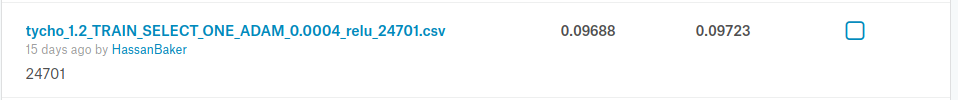
\includegraphics[width=\linewidth]{images/tycho12_result.png}
    \caption{Kaggle submission result of Tycho1.2 network after 24701 training epochs.)}
   \label{fig:tycho-12-solution}
\end{figure}

Moreover, it is now known that normalizing the solution file will not work with ReLu activation in the final layer, hence will be omitted from now on.


\chapter{The Network: Tycho2} \label{tycho2}

%ReLU network, reduce underfitting, produces overfitting, dropout use

\begin{figure}[H]
  \centering
    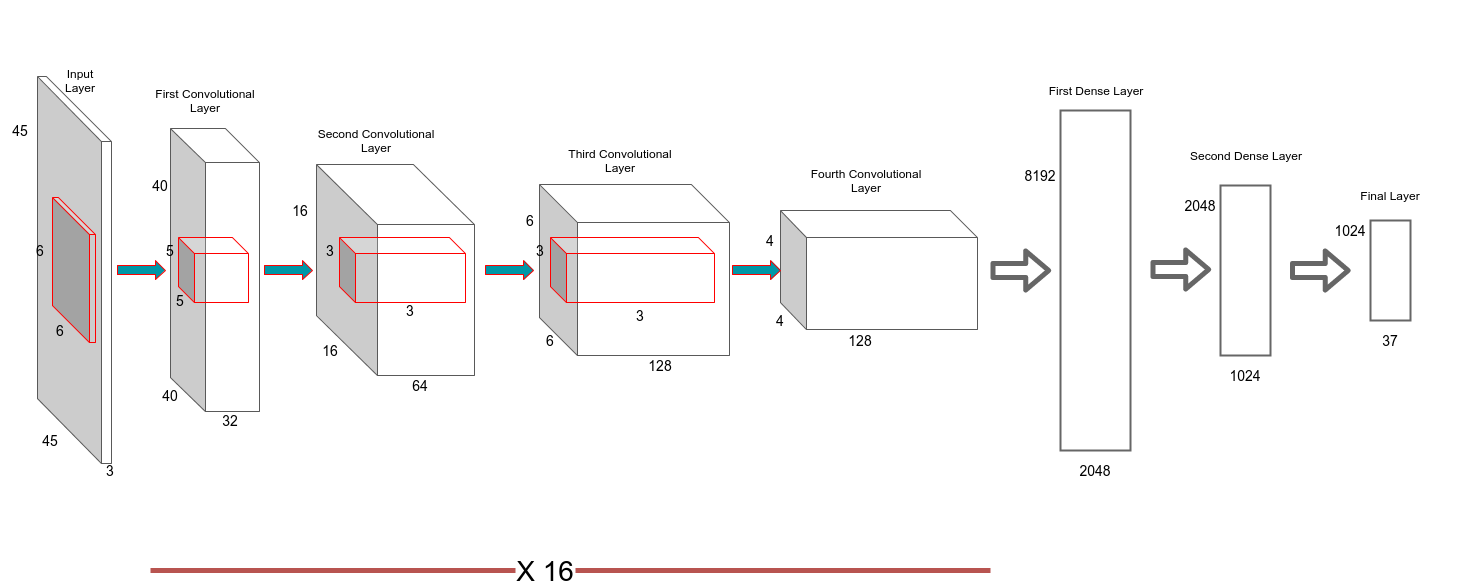
\includegraphics[width=\linewidth]{images/Tycho2.png}
    \caption{Diagram of the Tycho2 network}
   \label{fig:tycho-2-diagram}
\end{figure}

Seeing as the Tycho1, and Tycho1.2 networks both exhibit signs of under-fitting, we will need a network with more parameters to better fit the data. Hence, we develop a new network, titled Tycho2. This network will have larger fully connected layers so as to increase parameters, but will maintain the same configuration in the convolutional layers. Moreover, to achieve this, the Tycho2 will use a similar data pre-processing step as described by Sander Dieleman ~\cite{Sanders-GZ}.

Each input image is processed to generate 16 different augments as described in section \ref{aug-section}. All of these 16 augments are fed through the convolutional layers. After the augmented images go through the convolutional layers, the 16 augments of each image are concatenated into one bigger feature. This feature is then fed through two fully connected dense layers. This sees that the first dense layer is 16 times greater than that in Tycho1. This process is described in figure \ref{fig:tycho-2-diagram}.

\section{Validation}

The Tycho2 network is trained for 2000 epochs with a mini-batch of 16, just as the Tycho1.2 network was. This validation doesn't give way to much insight, but it does show that increasing the parameters does indeed improve the model, as both training and validation errors are lower after 2000 epochs.


\section{Training Details \& Results}

The Tycho2 model is trained on a mini-batch of 256 images, with each image augmented 16 times. A test interval of 5000 is set, meaning that after 5000 epochs, the model would generate a solution CSV file. 

The Tycho2 model's training error converges far quicker than Tycho1 and Tycho1.2 as can be seen with figure \ref{fig:tycho-2-12-graph}. However, this convergence begins to dip drastically after approximately 3000 epochs, which is highly unusually. By the time it reaches 5000 epochs, the training error is down to \(0.05191\), which extremely low. This leads to the assumption that this model is over-fitting. Hence the first solution file that was generated after 5000 epochs is tested. This produces an private RMSE value of \(0.10416\). This is evidence that this model is drastically over-fitting. Running it longer will not amount to any meaningful progress, hence the training is stopped. 


\begin{figure}[H]
  \centering
    
\includegraphics[width=\linewidth]{images/tycho2_results1.png}
    \caption{The test error of the Tycho2 Network after 5000 training epochs. Private score on the left and public score on the right.}
   \label{fig:tycho-2-result}
\end{figure}

\begin{figure}[H]
  \centering
    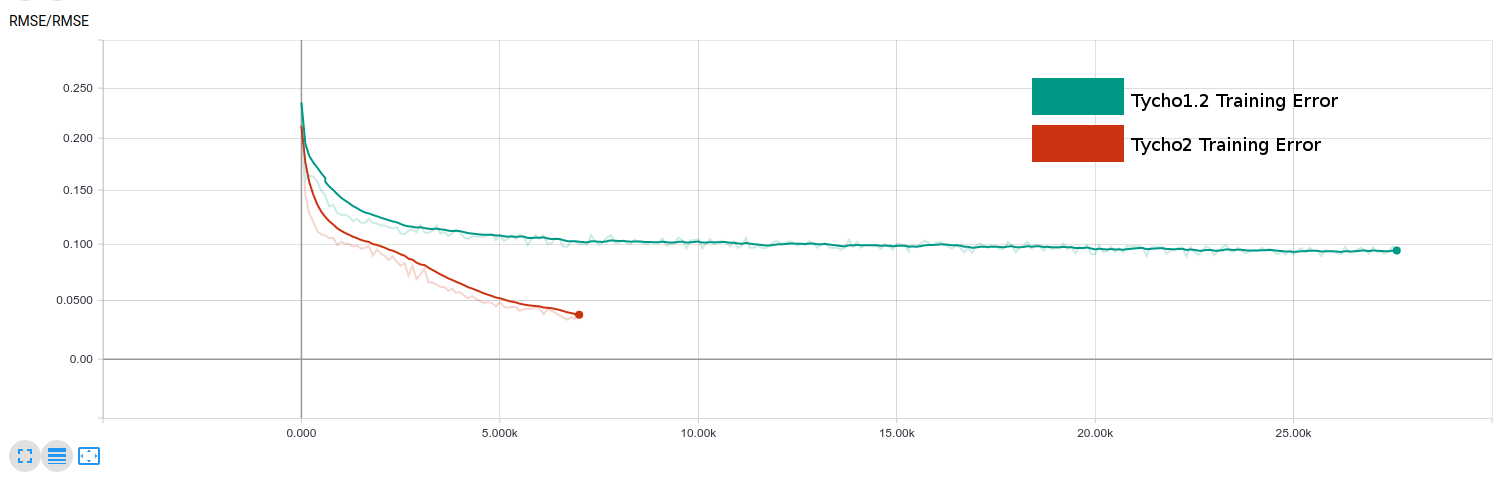
\includegraphics[width=\linewidth]{images/tycho2vs12.png}
    \caption{Graph of Tycho2 training error and Tycho1.2 training error}
   \label{fig:tycho-2-12-graph}
\end{figure}

\section{Conclusion}

We can conclude that although Tycho2 does produce a reasonable test error, running it further will be futile as it vastly over-fits. The key difference between the Tycho1.2 and Tycho2 architectures are the dense layers, hence we can conclude that the large dense layers in the Tycho2 network are what lead to this over-fitting. We will consider the effects of adding dropout regularization in the dense layers of the Tycho2 network in the next section.

\section{Tycho2 - Using Dropout Regularization} \label{tycho2-dropout}

So as to reduce over-fitting, the dense layers in the Tycho2 network are configured to have a dropout probability of 0.5 in the dense layers. This network will be trained from the beginning, using the same training configuration as before, and was allowed complete 15000 epochs of training.

\subsection{Results}

\begin{figure}[H]
  \centering
    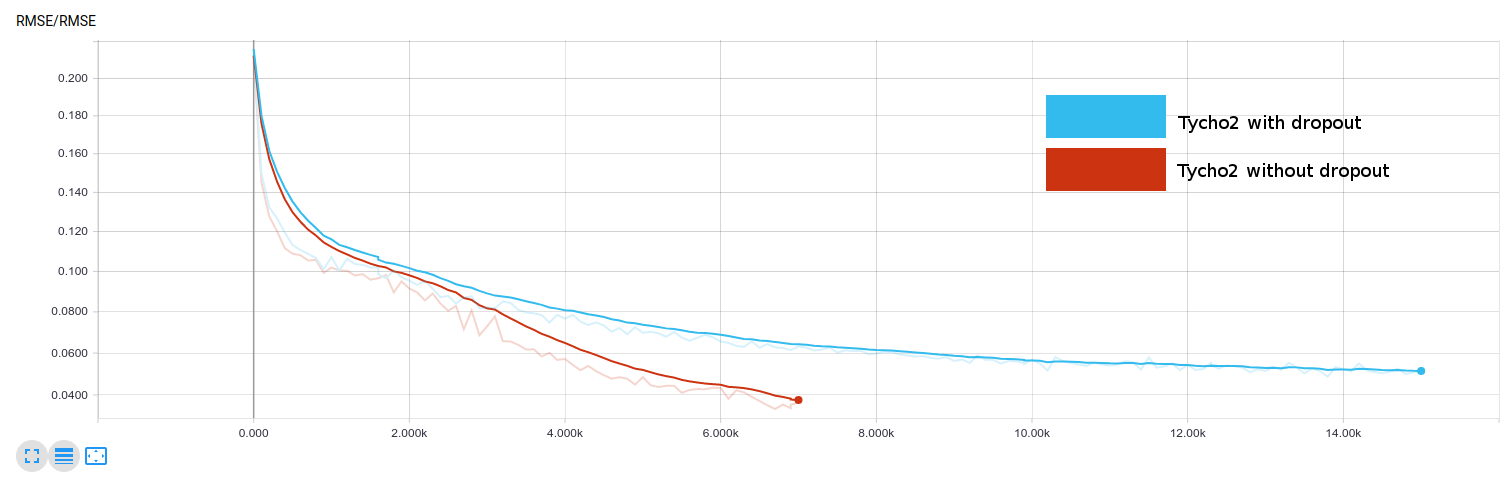
\includegraphics[width=\linewidth]{images/tycho2vsdropout.png}
    \caption{Graph of training errors of Tycho2 using dropout and Tycho2 without dropout.}
   \label{fig:tycho-2-dropout-graph}
\end{figure}


Looking at figure \ref{fig:tycho-2-dropout-graph} one can see that the effects of using dropout are clear from 200 epochs, and become even clearer after 2600 epochs. A solution file is generated after 5000 training epochs, which results in a test error of 0.10175, while the training error at 5000 epochs is 0.07373. 

\begin{center} \label{tycho2-results-table}
 \begin{tabular}{||c | c | c||} 
 \hline
 Training Epoch & Training Error & Validation Error \\ [0.5ex] 
 \hline\hline
 5000 & 0.07373 & 0.10175\\ 
 \hline
 10000 & 0.05693 & 0.10257\\
 \hline
 15000 & 0.05114 & 0.10300\\
 \hline
\end{tabular}
\end{center}
\begin{center}
\bigskip
Results of the Tycho2 network with a dropout probability of 0.5 in the dense layers
\end{center}


\subsection{Conclusion}

It is evident that dropout has significantly reduced over-fitting in the Tycho2 network, however it is still not enough. The dense layers in this network simply have too many units. Hence we will reduce the number of units in the dense layers of the next network.

\chapter{The Network: Tycho3} \label{tycho3}

%Maxout network, reduce underfitting, produces overfitting, not as much as ReLu, dropout use

Seeing as these large ReLu layers are contributing to a great amount of over-fitting, we will instead consider using maxout layers as described by Goodfellow et al ~\cite{maxout}. Maxout layers are very simple in principle but can be very powerful. In effect it is a variation of ReLu activation, whereby the weight is applied the inputs, the bias is added, and then the maximums of the selected neurons are taken, as described in \ref{eq:maxout}. Moreover, an interesting feature of maxout is that is found to learn the activation function of the layer that precedes it ~\cite{maxout}. In our case, the layer that precedes the first maxout layer is a convolutional layer with a ReLu activation function. 

\begin{equation}
    f(x)=max(x_0, x_1)
    \label{eq:maxout}
\end{equation}

Maxout is expected to be more effective than just using ReLu as it picks out the most meaningful (maximum) inputs to activate across all neurons, as this is a fully connected implementation. Whereas ReLu is restricted is more sparse, it either outputs 0, or a value that is greater 0.

The Tycho3 network is similar to the Tycho2 network, except the first and second dense layers are no longer ReLu layers, but instead maxout layers. The number of units the Tycho3 network contains in the maxout layers is less than the number of ReLu units in the corresponding layers of the Tycho2 network. This is because maxout is more computationally intensive than ReLu, which would slow down training greatly. Moreover, as we saw with the Tycho2 network, the large number of parameters in the dense layers leads to a vast amount of over-fitting. The Tycho3 network is visualized in figure \ref{fig:tycho-3-diagram}

\begin{figure}[H]
  \centering
    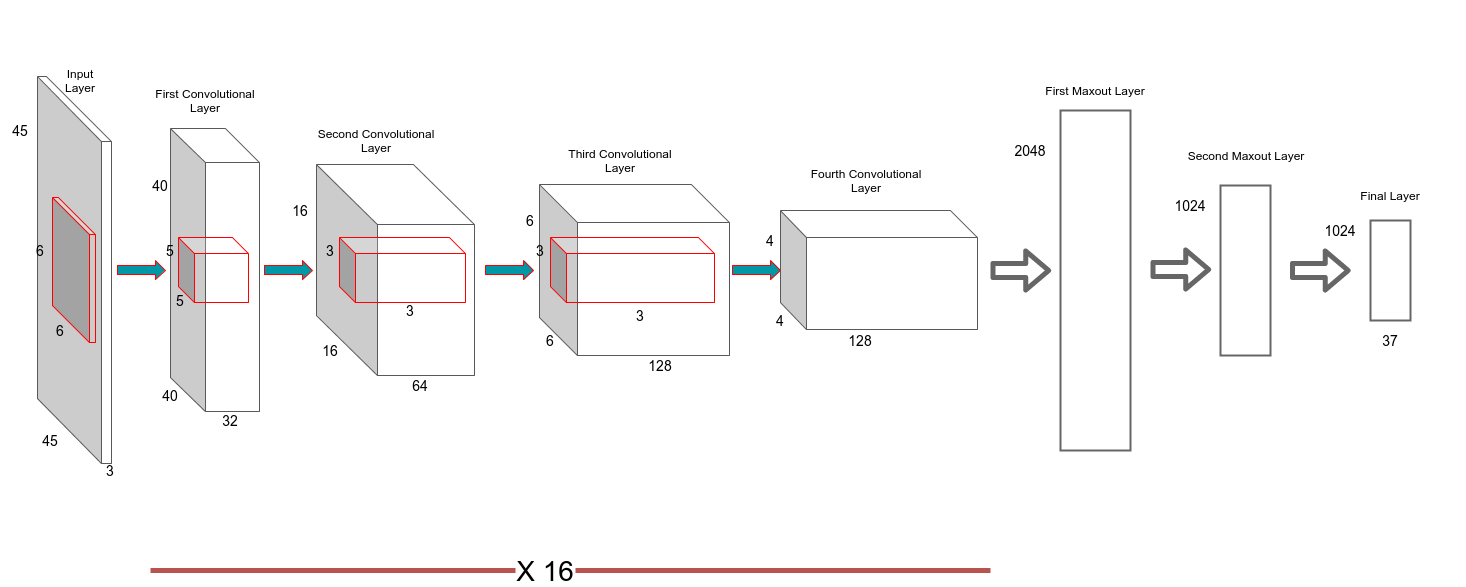
\includegraphics[width=\linewidth]{images/Tycho3.png}
    \caption{Diagram of the Tycho3 network}
   \label{fig:tycho-3-diagram}
\end{figure}


\section{Validation}

As can be seen from table \ref{val-table-1}, the Tycho3 network is trained for 2000 epochs on a mini-batch of 16, taking the validation and training errors every 100 epochs. In validation, the Tycho3 network outperforms the Tycho1.2 network, and also the Tycho2 network slightly. However as we know from training the Tycho2 network, the early stages of the Tycho2 network are not perfectly reflective of it's overall performance as it starts to noticeably over-fit after 3000 epochs. 

\begin{center} \label{val-table-1}
 \begin{tabular}{||c | c | c||} 
 \hline
 Network & Training Error & Validation Error \\ [0.5ex] 
 \hline\hline
 Tycho1 & 0.1517 & 0.1479\\ 
 \hline
 Tycho1.2 & 0.1181 & 0.11452\\
 \hline
 Tycho2 & 0.1285 & 0.1217\\
 \hline
 Tycho3 & 0.1219 & 0.1209\\
 \hline
\end{tabular}
\end{center}

\section{Training Details \& Results}

The Tycho3 network is set to train for 15000 epochs on a mini-batch of 256, generating a CSV test solution every 5000 epochs. Upon the generation of the first solution file at the \nth{5000} epoch, the Tycho3 network exhibits signs of over-fitting, resulting in a training error of 0.09943, and a test error of 0.10293. This is not as drastic as Tycho2, but nonetheless, not negligible. This was left run for the whole 15000 epochs, completing with a training error of 0.08590, and a test error of 0.09833.

\section{Conclusion}

The training of the Tycho3 network concludes that using maxout layers with less units than the ReLu layers used in the Tycho2 network does significantly reduce over-fitting, but not entirely. However, it does still outperform the Tycho1.2 network. Furthermore, we can conclude that this network does stand to benefit from the use of dropout, hence this will be implemented in section \ref{tycho3-dropout} 

\section{Tycho3 - Using Dropout Regularization} \label{tycho3-dropout}

A dropout probability of 0.5 is implemented in the maxout layers of the Tycho3 network. This is trained from the beginning for 15000 epochs on a mini-batch of 256. The effects of dropout become apparent only after 500 epochs, when comparing the error graph of the Tycho3 network with dropout and without dropout. The convergence in the graph of the Tycho3 network with dropout begins to slow down quicker. This can be seen in figure \ref{fig:tycho-3-dropout-graph}

\begin{figure}[H]
  \centering
    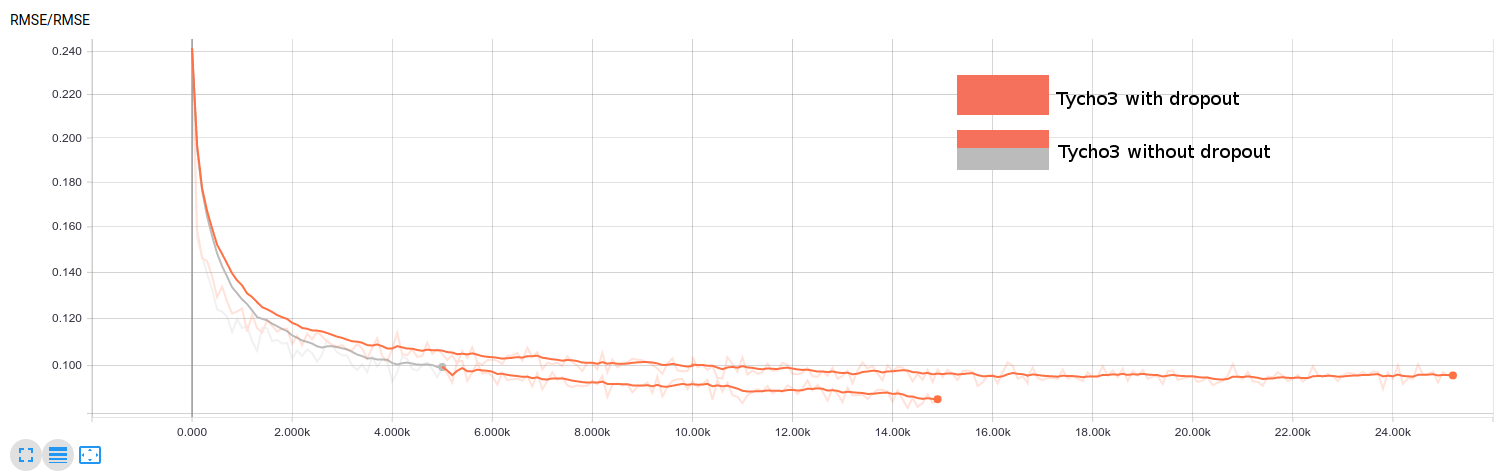
\includegraphics[width=\linewidth]{images/tycho3vsdropout.png}
    \caption{Graph of Tycho3 with dropout training error and Tycho3 without dropout training error. \textbf{N.B.} The graph for the Tycho3 error without the use of dropout is split into two colours, grey and orange. This is because a code change was made that resulted in the graphs having different names, hence TensorBoard reads them as two separate graphs.}
   \label{fig:tycho-3-dropout-graph}
\end{figure}

After 15000 epochs the Tycho3 network (with dropout) results in a training error of 0.09526, and a test error of 0.09836, which is as expected. Now that over-fitting has been reduced greatly, we can use the training error as a good assessment of the models progress. 

Looking at figure \ref{fig:tycho-3-dropout-graph}, we can see that when it reaches the \nth{10000}, it begins to slow down it's progress. However, just like the Tycho1.2 network, this is left run for 7 days, up till the \nth{25000} epoch to better evaluate the model. At epoch 25000, it reaches a training error of 0.9735, and a test error of 0.09747, which is slightly less than what the Tycho1.2 model produced, which was 0.09688, which is surprising.

\section{Conclusion}

We can conclude that using dropout on the Tycho3 network does have a significantly positive effect on the training error. Furthermore, we can conclude that this network performs about the same as the Tycho1.2 network, meaning that we could still be making this model a bit overly complex. Cutting down the number of units in the maxout layers would be a starting point.


\chapter{Study: Varying Number Of Convolutional Layers Experiment} \label{conv-exp}

This project has focused heavily on the dense layers of deep convolutional neural networks but has not experimented with the convolutional layers themselves. Hence this experiment aims to study the effects of having various numbers of convolutional layers. In practice, more convolutional layers will be subject to the same problems dense layers are, these problems being over-fitting and under-fitting. 


\section{Experiment Description}

We have been currently working with four convolutional layers, hence will experiment the effects of a network with three convolutional layers and a network with 5 convolutional layers. 

We will maintain the same data pre-processing method as Tycho1 and Tycho1.2 as described in section \ref{tycho-data}, as well as keeping to same dense layers as Tycho1.2. This is because so far the Tycho1.2 network has proven to be the most effective, and does not exhibit signs of over-fitting. 

We will train the three different convolutional neural networks described in this chapter for 2000 epochs, on a mini-batch of 16, taking training and validation errors every 50 epochs. 

The three-convolutional-layer and five-convolutional-layer implementations will be described in this chapter, but refer to chapter \ref{tycho1-arch} for the four-convolutional-layer implementation. 

\subsection{Three Convolutional Layers}

\begin{figure}[H]
  \centering
    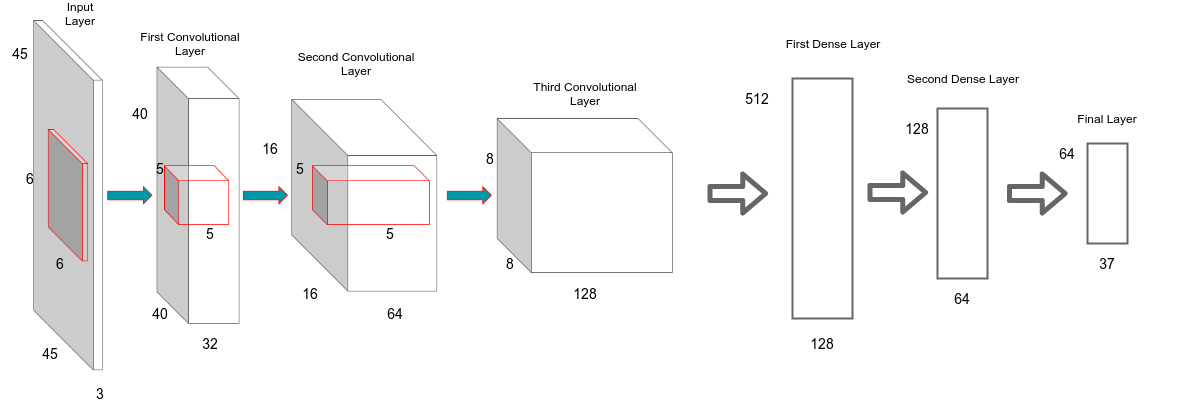
\includegraphics[width=\linewidth]{images/Tychoconv3.png}
    \caption{Diagram of a variation of the Tycho1.2 network with 3 convolutional layers instead of 4}
      \label{fig:conv3}
\end{figure}


The three convolutional layer architecture will contain a filter of size \(6\times6\), and and output size of 32 in the first layer. The second layer will contain a filter size of \(5\times5\), and an output size of 64. The last convolutional layer will contain a filter size of \(5\times5\), and an output size of 128. All convolutional layers will be followed by a \(2\times2\) max-pooling layer. This can be seen in figure \ref{fig:conv3}.

\subsection{Five Convolutional Layers}


\begin{figure}[H]
  \centering
    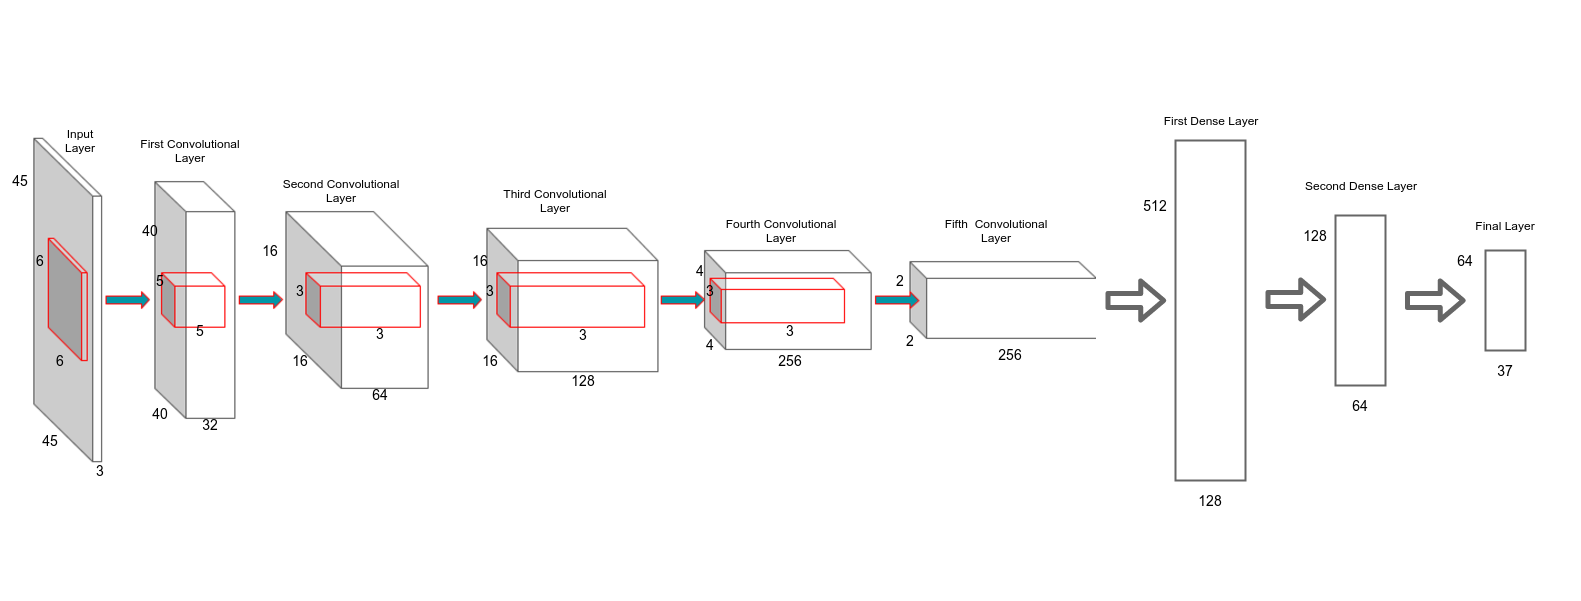
\includegraphics[width=\linewidth]{images/conv5.png}
    \caption{Diagram of a variation of the Tycho1.2 network with 5 convolutional layers instead of 4}
       \label{fig:conv5}
\end{figure}

This implementation contains five convolutional layers, and is described in figure \ref{fig:conv5}. The first layer contains a filter of size \(6\time6\), and an output size of of 32. The second layer has a filter size of \(5\times5\), and an output size of 64. The third layer has a filter size of \(3\times3\), and an output size of 128. The fourth layer contains a filter of size \(3\times3\) and an output size of 256. The final convolutional layer contains a filter of size \(3\times\3\), and an output size of 512. All layers except the third and fourth are followed by max-pooling layers of size \(2\times2\).

\section{Results}

\begin{center} \label{val-table-conv}
 \begin{tabular}{||c | c | c||} 
 \hline
 Network & Training Error & Validation Error \\ [0.5ex] 
 \hline\hline
 Three Convolutional Layers & 0.1350 & 0.1396\\ 
 \hline
 Four Convolutional Layers & 0.1305 & 0.1480\\
 \hline
 Five Convolutional Layers & 0.1357 & 0.1416\\
 \hline
\end{tabular}
\caption{Experiment results after 2000 epochs.}
\end{center}

\begin{figure}[H]
  \centering
    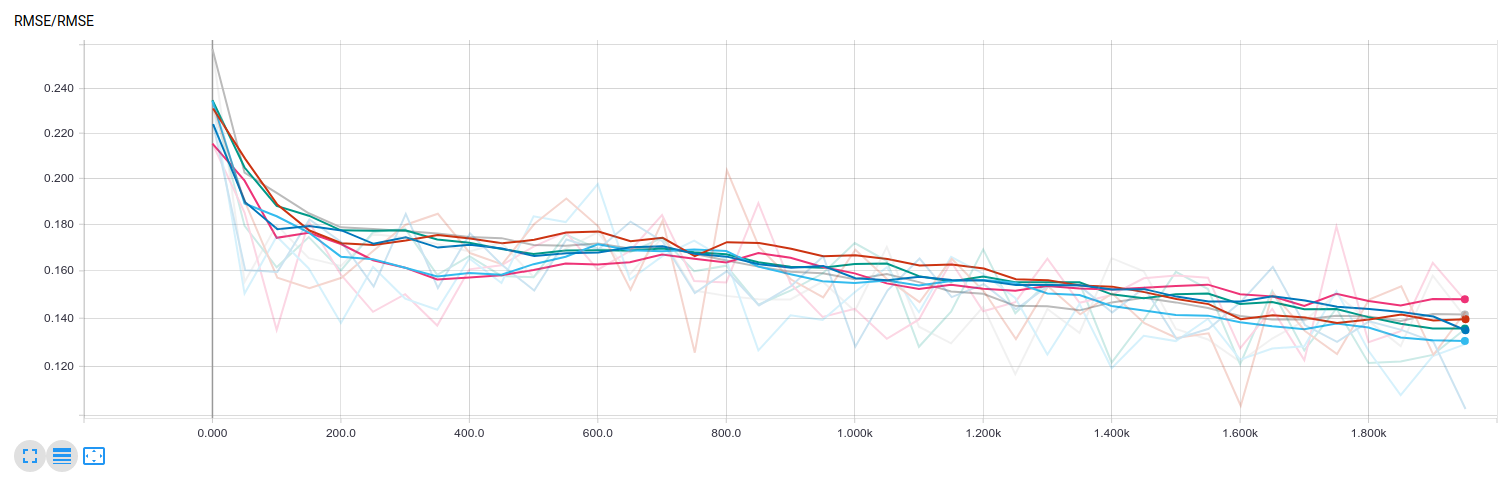
\includegraphics[width=\linewidth]{images/convgraph.png}
    \caption{Graph of of training and validation errors of all three networks. \textbf{N.B.} There is no legend in this graph as there is too many lines, and they are all behaving identically.}
      \label{fig:conv-graph}
\end{figure}

\section{Conclusion}

From the results gathered, we can conclude that there isn't a large difference between these networks. Although using four convolutional layers does do worse here, it is not by an amount that is drastic, especially as these networks only train for 2000 epochs. Moreover, by looking at how they converge, it is easy to see that there is no stark differences between these implementations. This makes sense when you consider the data at hand, as the galaxies in the images are generally uniform. Moreover, galaxy shapes are quite regular, and not too complex. Hence, it would most likely be recommended to go forward with three convolutional layers rather than four, simply because it would be more computationally efficient.

\chapter{Project Conclusion}


\section{Goals Achieved}

Looking back at section \ref{goals}, we can show that we have indeed achieved many of the aims and goals. We have successfully analysed the data. We successfully compared learning optimization algorithms and found an optimal learning rate. We studied the activation functions highlighted, and tackled the issues of over-fitting and under-fitting. 

We did not achieve the aim of developing and studying the winning solution \ref{winning-sol}, although the Tycho3 model is similar in many ways. This is because time did not permit it, as these deep networks are very timely to train. Moreover, one of the  aspects of Dieleman's solution could not be implemented using the TensorFlow Python API. This is the custom activation function written in the final layer of the network, as detailed in section \ref{tycho1-arch}. Furthermore. it is worth mentioning that the student did not understand a detail in the winning solution, in regards to how many units used in the maxout layers. In anticipation of achieving this goal, the student contacted Sander Dieleman so as to get clarification on this detail via email. This email exchange can be found in appendix \ref{email}.

However, we validated and trained 4 networks. Most Notably, the Tycho1.2 network and the Tycho3 network achieved a test error of \(0.09688\) and \(0.09747\) respectively. This would rank the Tycho1.2 model in the \nth{38} spot, and the Tycho3 model in \nth{39} spot. This achieves our goal of producing a solution that would rank in the top 50 of the leader board. 

Notably, all the networks we trained beat one of the solutions studied in this project, Fang ~\cite{Fang}, who achieved a testing error of 0.11150. This is interesting as although Fang's implementation did use a pre-trained convolutional neural network, the results were averaged with various other methods. Fang explains that he opted out of training a deep convolutional network as it is time and resource expensive, which is a correct assessment. This clearly shows the effectiveness of deep convolutional networks for image recognition.

Moreover, this high performance can be attributed to a number of factors. Firstly, the use of the Adam optimizer is extremely effective here, however this algorithm was not available to any of the competition entrants as it was first published by Kingma et al ~\cite{Kingma} in 2015, and this competition was launched and ended in 2014. Furthermore, the use of a machine with a powerful GPU, such the Nvidia GTX 1080 used in this project, drastically increases the time it takes to train these networks. An advantage of this meant that the student can train these networks for 7 days and get these high results. However, the most crucial factor to consider is that educational resources are becoming more and more novice friendly, where as it would have been far more difficult to understand these concepts and achieve these results in even 2014.

Furthermore, the practical work involved in this project proves that the student has learned and gained valuable insight in developing and working with deep convolutional neural networks.

\section{Recommended Improvements}

Although many of the highlighted topics have been studied, the results prove that, time permitting, there is yet far more options to consider so as to produce lower levels of error. For instance, what we haven't studied is a network that uses a combination of ReLu and maxout layers, as we have seen that both of these layers produce good models.

Furthermore, it would be very interesting to ensemble some of these networks so as to carry out model averaging in an effort to lower the error. This is a standard practice in Kaggle competitions, however, it is particularly tricky to implement with TensorFlow, as there is no set way of doing it, hence would involve plenty of development.

Another interesting study would be to try to implement and study a winning model from another Kaggle competition such as the Kaggle Plankton classification by Dieleman et al ~\cite{Sanders-P}. This was a recommendation by Sander Dieleman from the email exchange from appendix \ref{email}. 

Moreover, a recommended improvement would be to use transfer learning to try to improve this model. This would involve taking a pre-trained network, which there is plenty of, and using some of the it's early layers in a new model. This should speed up the training time, but will require a bit of tweaking to get optimal results. 

Notably, we have not carried out any study on the colour in this data. This is because it did not seem overly important initially. However, reaching the limits hit with Tycho1.2 network and the Tycho3 network, it seems apparent that more can be done in the data processing step. There are numerous data processing and augmentation methods that can be studied an used. In fact there has already been some study done on the impact of colour when it comes to classifying galaxy morphology of the first Galaxy Zoo dataset by Lintott et al. ~\cite{Lintott}. This study finds that the colour in the images does impact the classification done by humans, however it is not critical but still useful. 

It would also be highly recommended to learn C++ so as to use the TensorFlow C++ API, as it proves to offer much more flexibility than the Python API.

Furthermore, it would be highly interesting to use this dataset to experiment with capsule networks, as although this an old theory ~\cite{cap1}, it has seen some very recent developments in 2017 that have shown bench-marked results with either lower error than convolutional neural networks, or on par with them ~\cite{cap2}. The GZ2 would be excellent for these types of networks as the first question asked in the flowchart is "Could this be a disk viewed edge-on?", and capsule networks are designed to be effective at learning patterns that are in a frame of reference, meaning that they should theoretically be good at learning whether there is a disk being viewed from all kinds of directions. 
\chapter{Closing Remarks}

Upon taking up this project, I had no prior experience in working with machine learning. I took on this project as I wanted to gain experience in this field. Moreover, this project was very enticing as it is less so a development based project and more of a research based project. Finding this as my only opportunity as an Undergraduate student to take on a research type project, I figured I should take it as I already have experience in development based projects.

I found this field to contain a very steep learning curve, I do think that this will improve over time as more educational resources become available. However, having the opportunity to get this level of experience in the early stages of this field is very valuable. I am confident that the effort I have put into this project has given me a level of insight that I could not achieve through theory alone. I am very proud of the work I achieved in this project and would credit most of it to the level of research I had done early on.

Now that I have enough experience in working with TensorFlow, I am looking to revisit my original idea of a Python dictionary based neural network builder using TensorFlow as an open-source project. I feel that if one doesn't have to worry about the development aspect, it will be easier to translate some of the solutions detailed in research publications and Kaggle competitions for beginners, rather than having to learn a new framework that follows a development style that is very different to most conventions. 

\appendix
\chapter{Optimizer \& Learning Rate Study Graphs}

The resultant TensorBoard graphs from the learning optimization algorithm study and learning rate search from chapter \ref{study1}.

\begin{figure}[H]
  \centering
    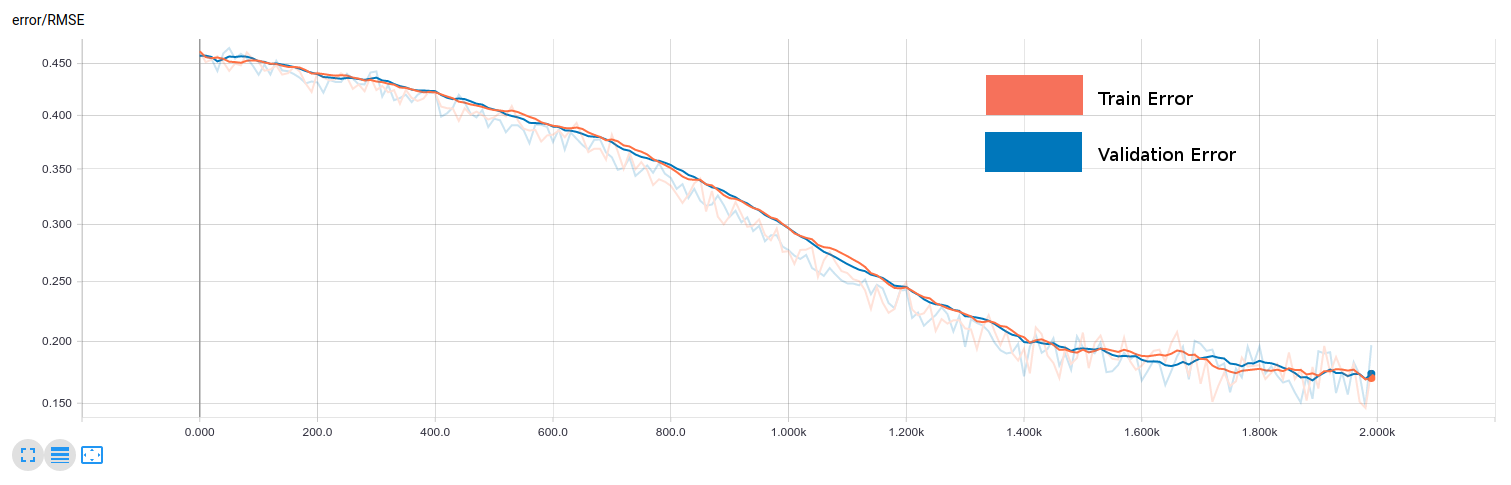
\includegraphics[width=\linewidth]{graphs/A/tycho_1_SGD_04_sigmoid_train.png}
    \caption{Graph of the Tycho1 network using SGD with a learning rate of 0.04}
\end{figure}

\begin{figure}[H]
  \centering
    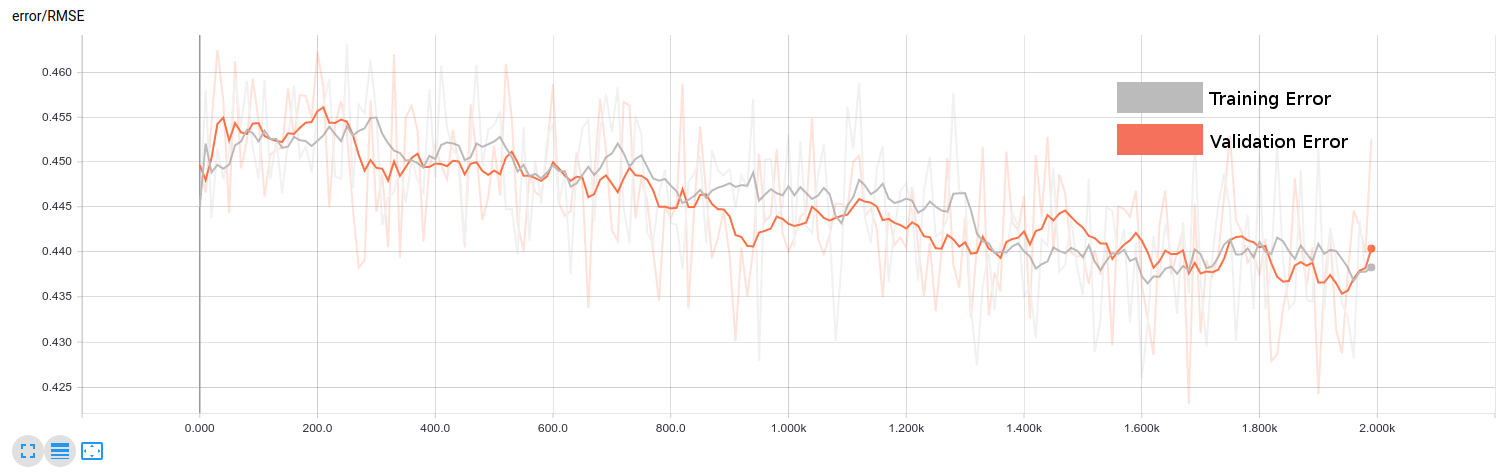
\includegraphics[width=\linewidth]{graphs/A/tycho_1_SGD_004_sigmoid.png}
    \caption{Graph of the Tycho1 network using SGD with a learning rate of 0.004}
\end{figure}

\begin{figure}[H]
  \centering
    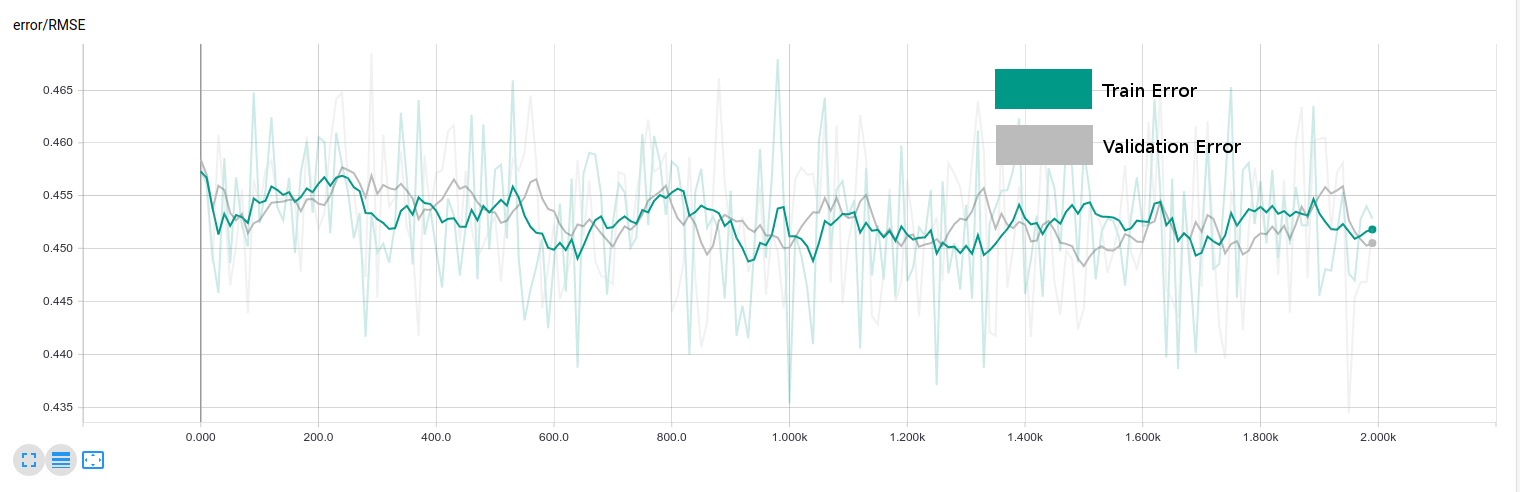
\includegraphics[width=\linewidth]{graphs/A/tycho_1_SGD_0004_sigmoid.png}
    \caption{Graph of the Tycho1 network using SGD with a learning rate of 0.0004}
\end{figure}

\begin{figure}[H]
  \centering
    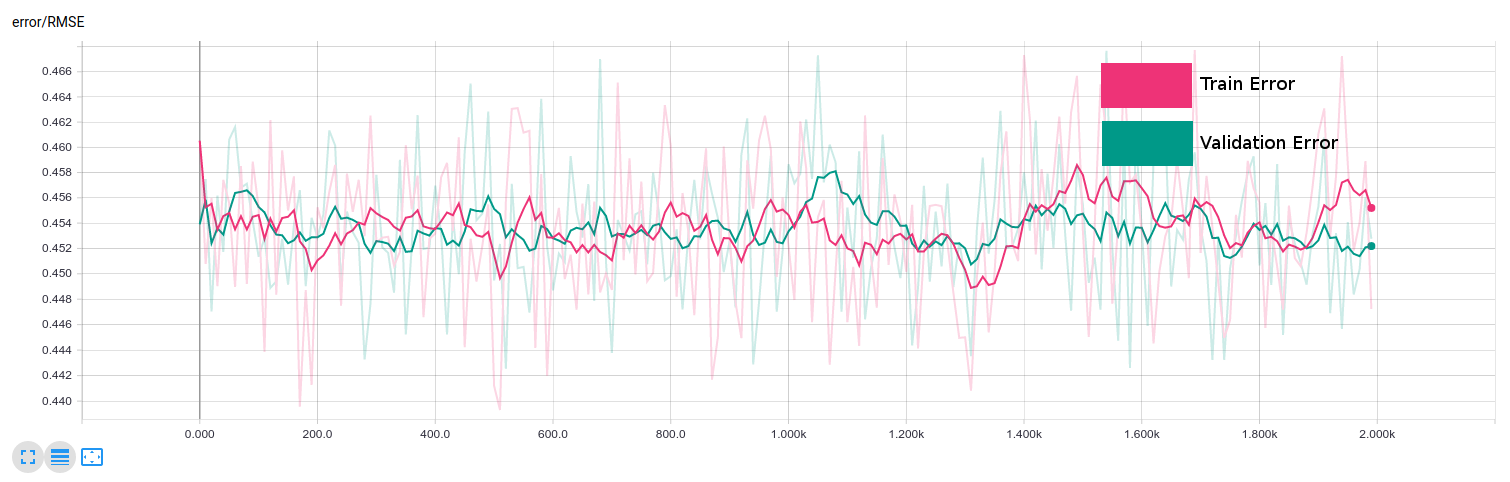
\includegraphics[width=\linewidth]{graphs/A/tycho_1_SGD_0001_sigmoid.png}
    \caption{Graph of the Tycho1 network using SGD with a learning rate of 0.0001}
\end{figure}

\begin{figure}[H]
  \centering
    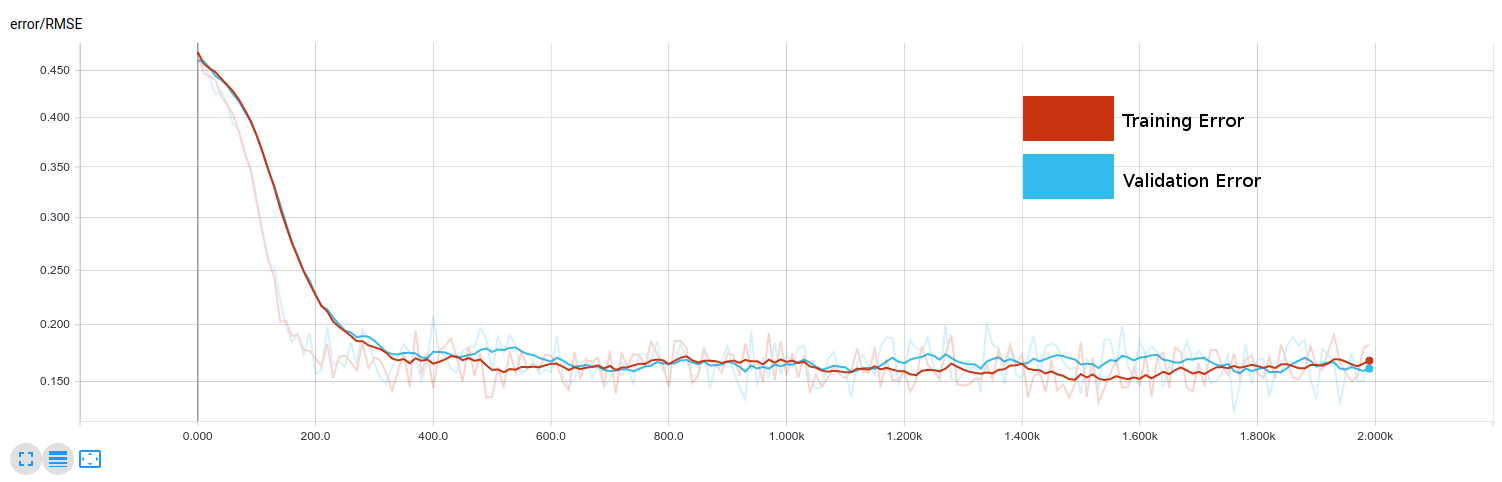
\includegraphics[width=\linewidth]{graphs/A/tycho_1_NESTEROV_04_sigmoid.png}
    \caption{Graph of the Tycho1 network using SGD withe nesterov momentum with a learning rate of 0.04}
\end{figure}

\begin{figure}[H]
  \centering
    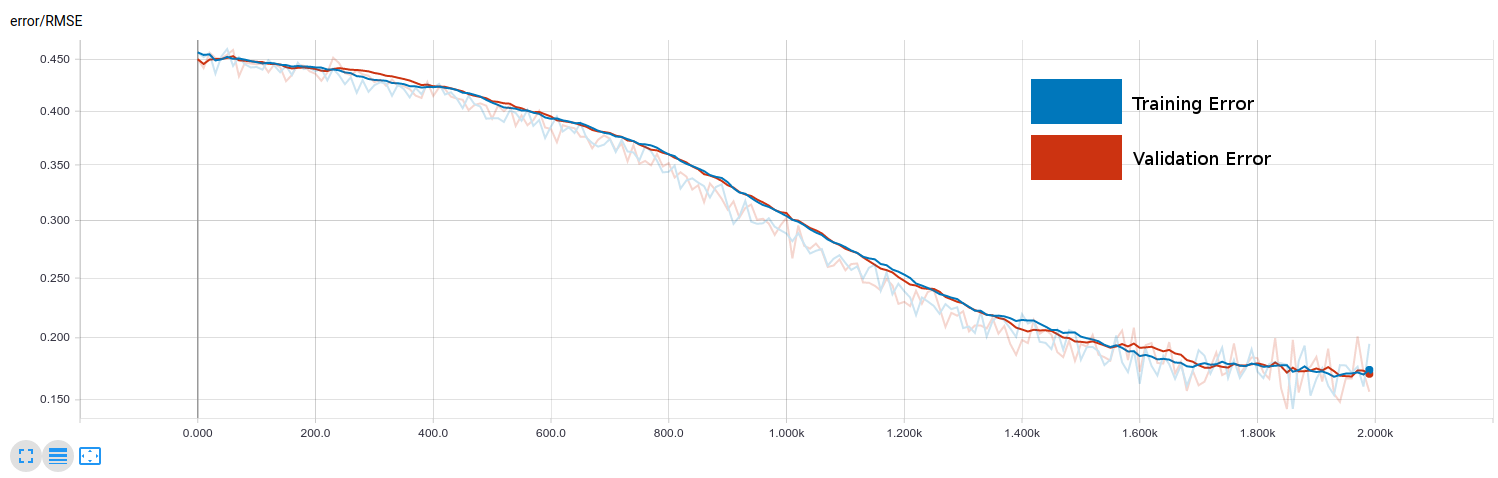
\includegraphics[width=\linewidth]{graphs/A/tycho_1_NESTEROV_004_sigmoid.png}
    \caption{Graph of the Tycho1 network using SGD withe nesterov momentum with a learning rate of 0.004}
\end{figure}

\begin{figure}[H]
  \centering
    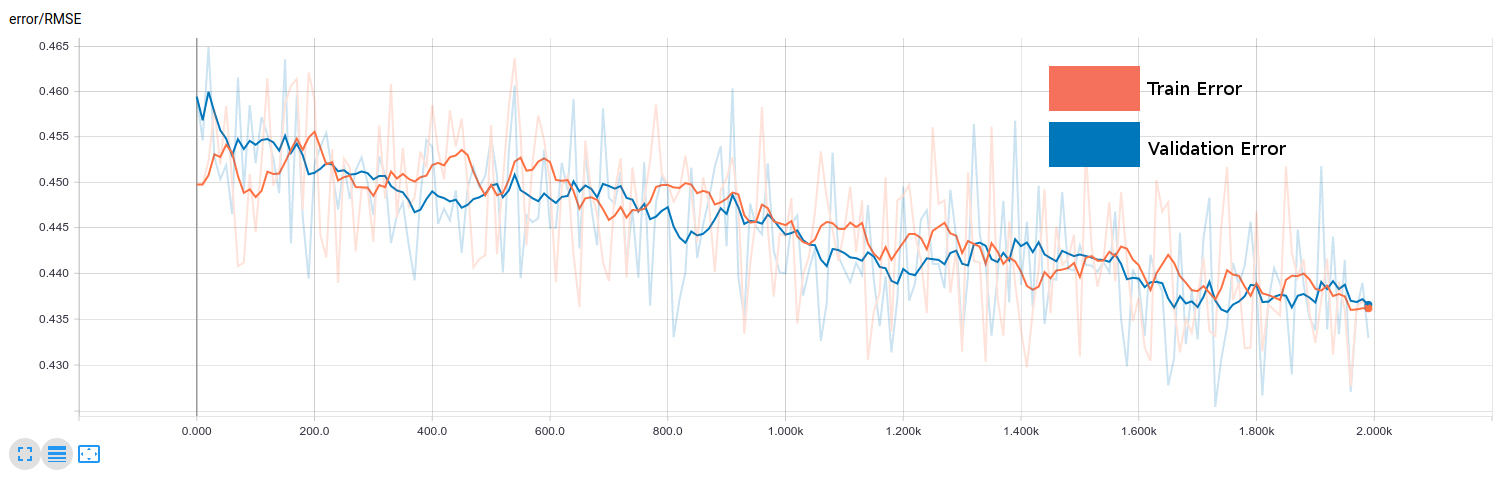
\includegraphics[width=\linewidth]{graphs/A/tycho_1_NESTEROV_0004_sigmoid.png}
    \caption{Graph of the Tycho1 network using SGD withe nesterov momentum with a learning rate of 0.0004}
\end{figure}

\begin{figure}[H]
  \centering
    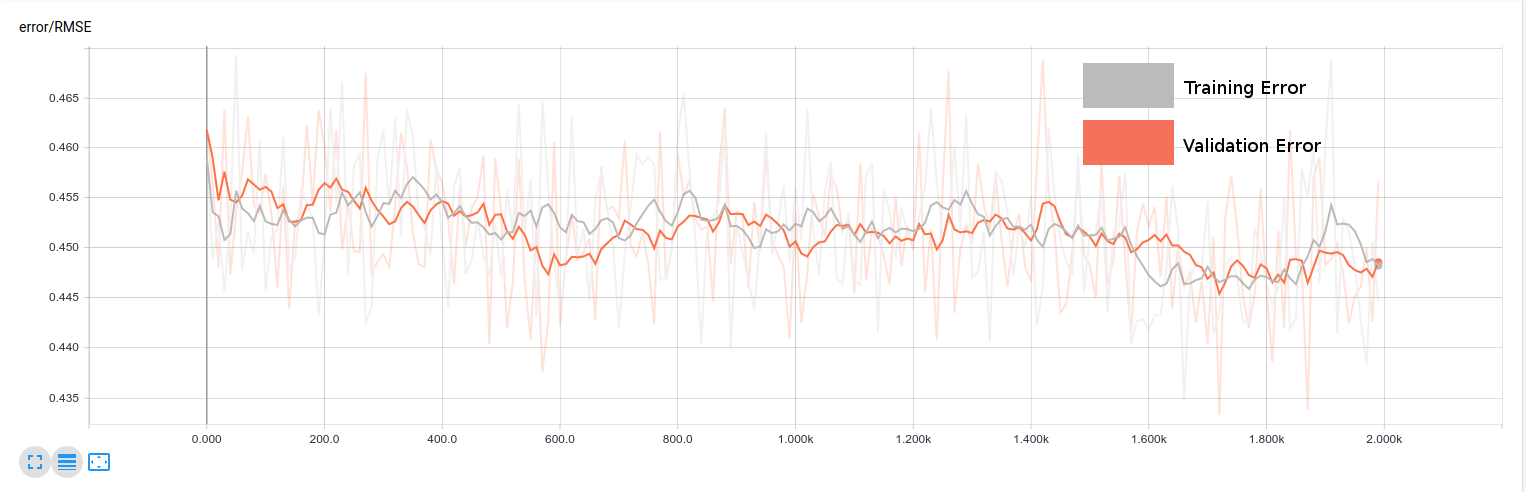
\includegraphics[width=\linewidth]{graphs/A/tycho_1_NESTEROV_0001_sigmoid.png}
    \caption{Graph of the Tycho1 network using SGD withe nesterov momentum with a learning rate of 0.0001}
\end{figure}

\begin{figure}[H]
  \centering
    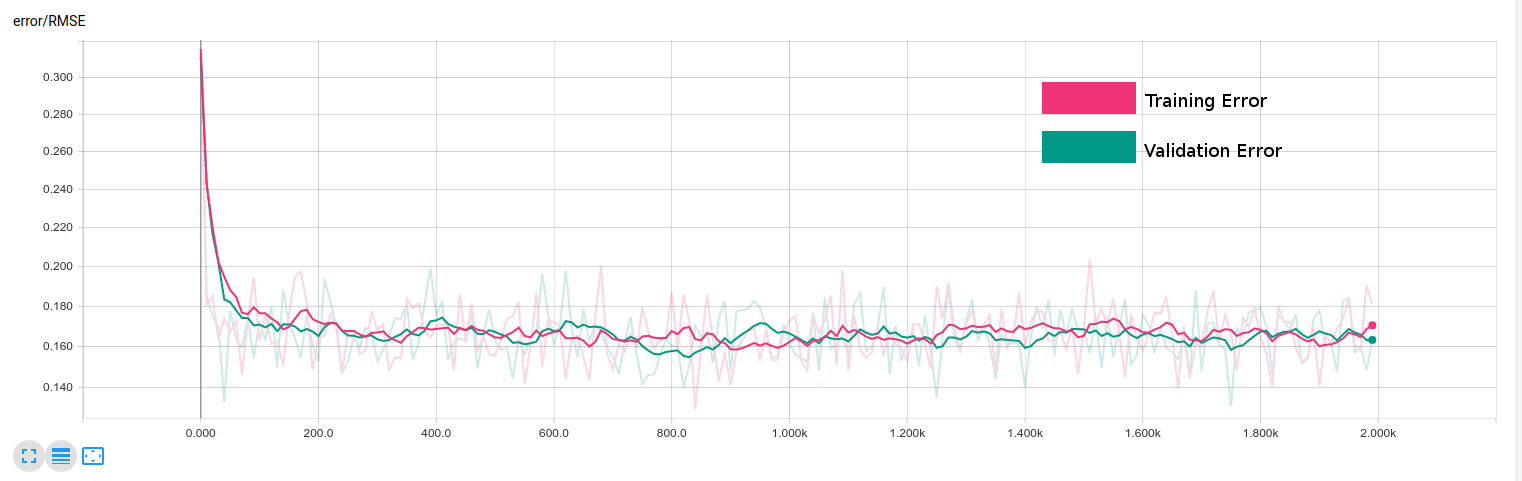
\includegraphics[width=\linewidth]{graphs/A/tycho_1_ADAM_04_sigmoid.png}
    \caption{Graph of the Tycho1 network using the Adam optimiser with a learning rate of 0.04}
\end{figure}

\begin{figure}[H]
  \centering
    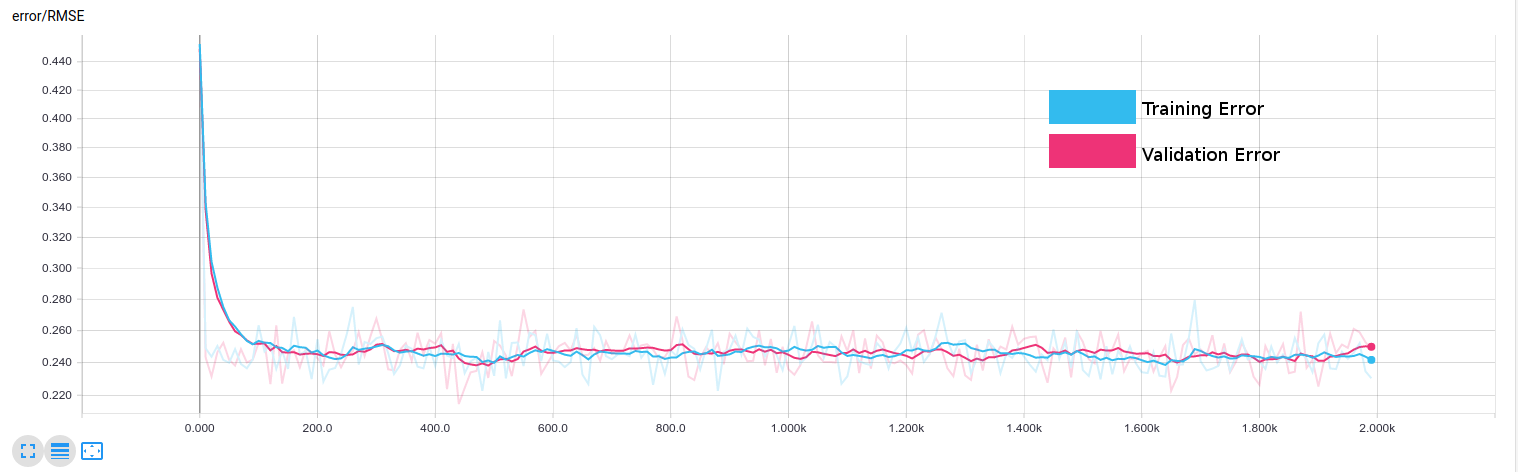
\includegraphics[width=\linewidth]{graphs/A/tycho_1_ADAM_004_sigmoid.png}
    \caption{Graph of the Tycho1 network using the Adam optimiser with a learning rate of 0.004}
\end{figure}

\begin{figure}[H]
  \centering
    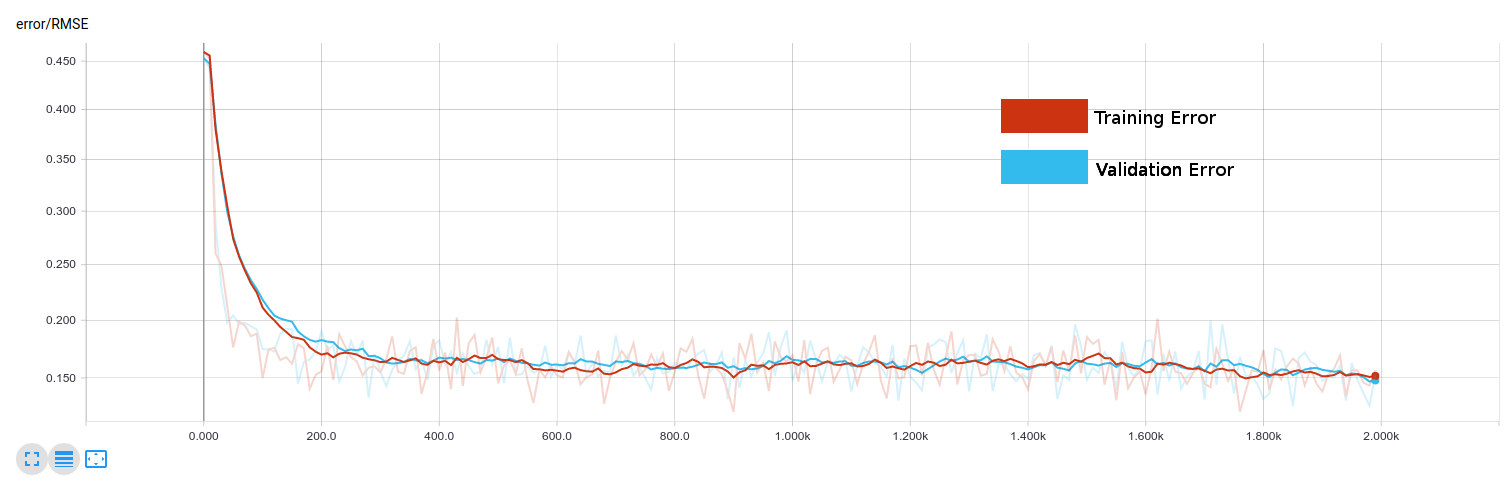
\includegraphics[width=\linewidth]{graphs/A/tycho_1_ADAM_0004_sigmoid.png}
    \caption{Graph of the Tycho1 network using the Adam optimiser with a learning rate of 0.0004}
\end{figure}

\begin{figure}[H]
  \centering
    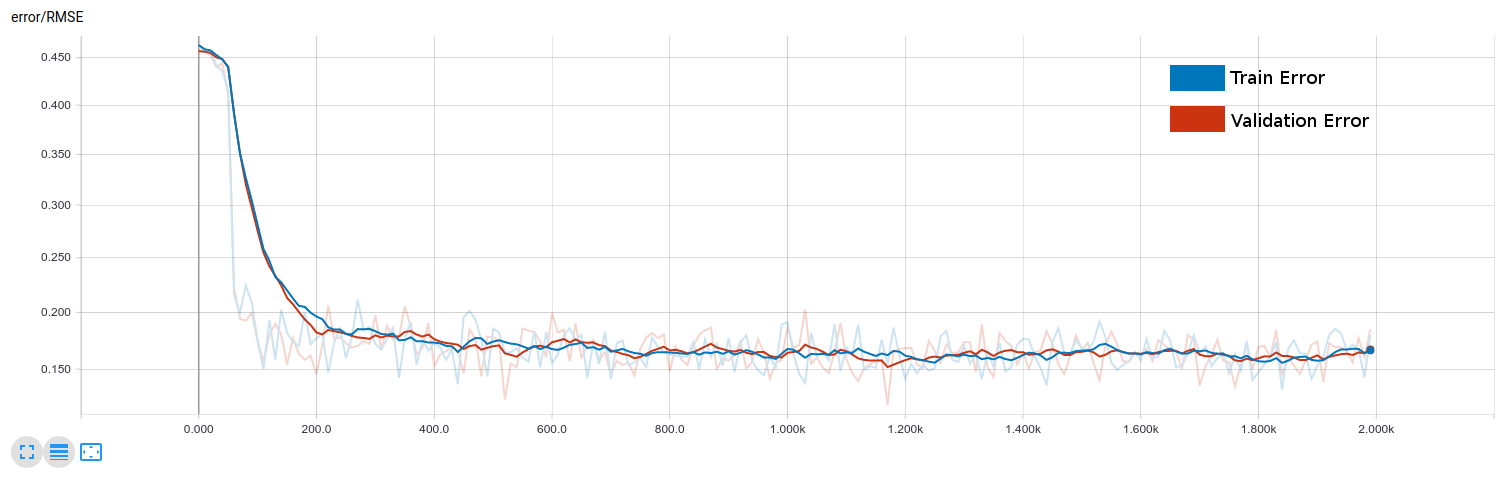
\includegraphics[width=\linewidth]{graphs/A/tycho_1_ADAM_0001_sigmoid.png}
    \caption{Graph of the Tycho1 network using the Adam optimiser with a learning rate of 0.0001}
\end{figure}

\begin{figure}[H]
  \centering
    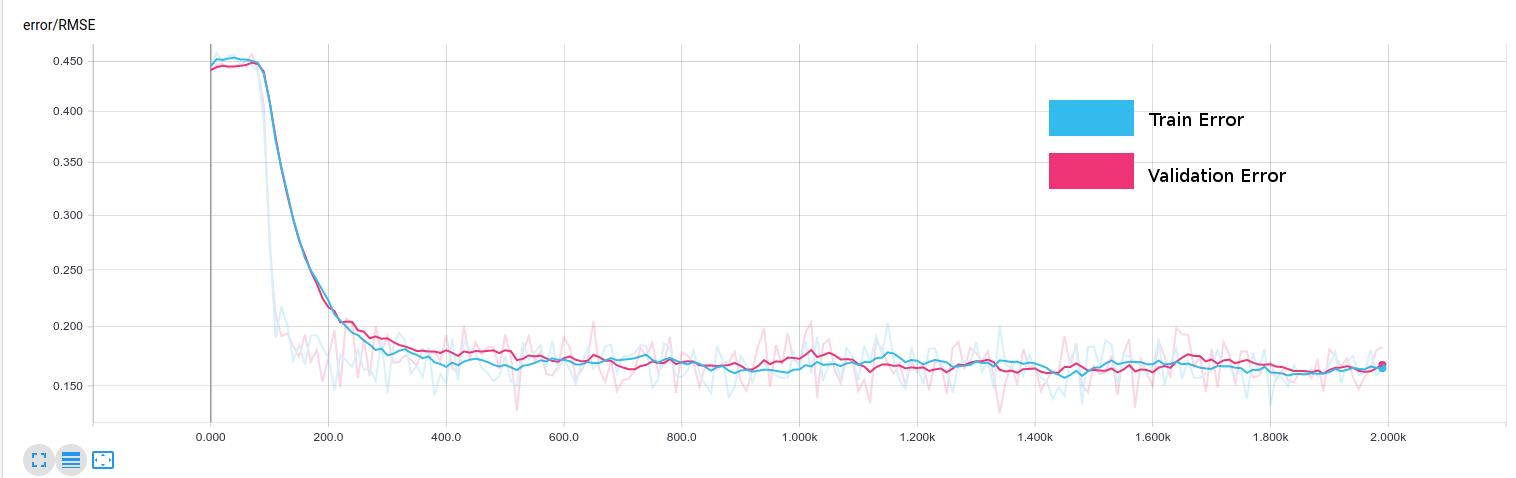
\includegraphics[width=\linewidth]{graphs/A/tycho_1_ADAM_4e-05_sigmoid.png}
    \caption{Graph of the Tycho1 network using the Adam optimiser with a learning rate of 0.00004}
\end{figure}

\begin{figure}[H]
  \centering
    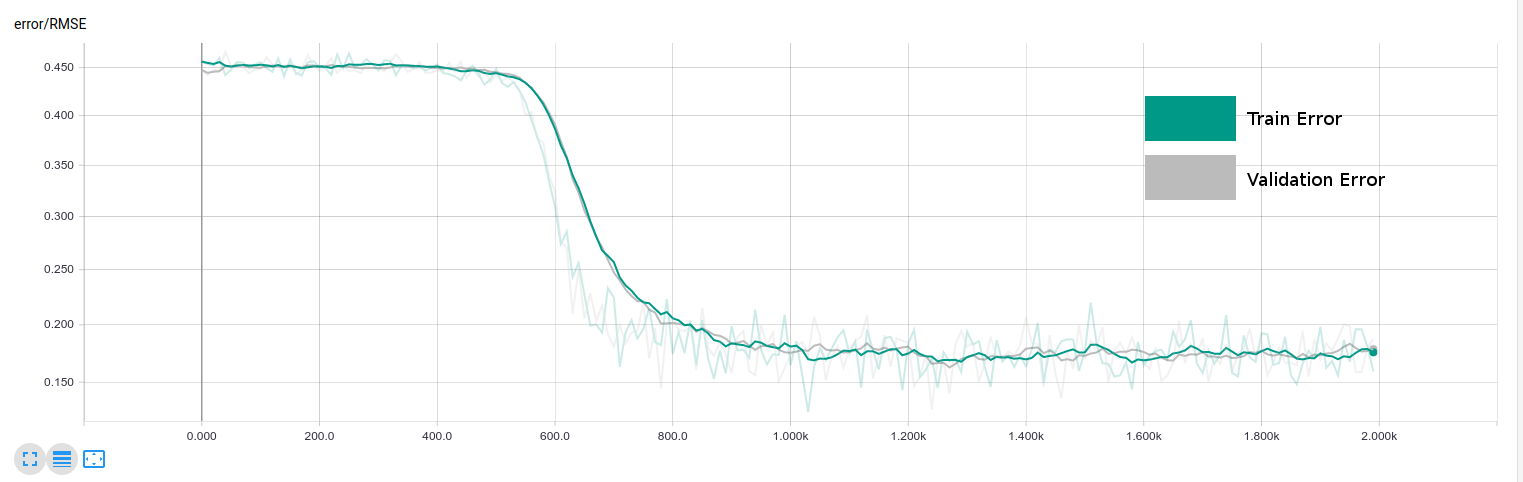
\includegraphics[width=\linewidth]{graphs/A/tycho_1_ADAM_4e-06_sigmoid.png}
    \caption{Graph of the Tycho1 network using the Adam optimiser with a learning rate of 0.000004}
\end{figure}

\chapter{Tycho1 Graphs}

The resultant TensorBoard graph of the training error, from the training of the Tycho1 network, from chapter \ref{tycho1}.
 
\section{Training}
\begin{figure}[H]
  \centering
    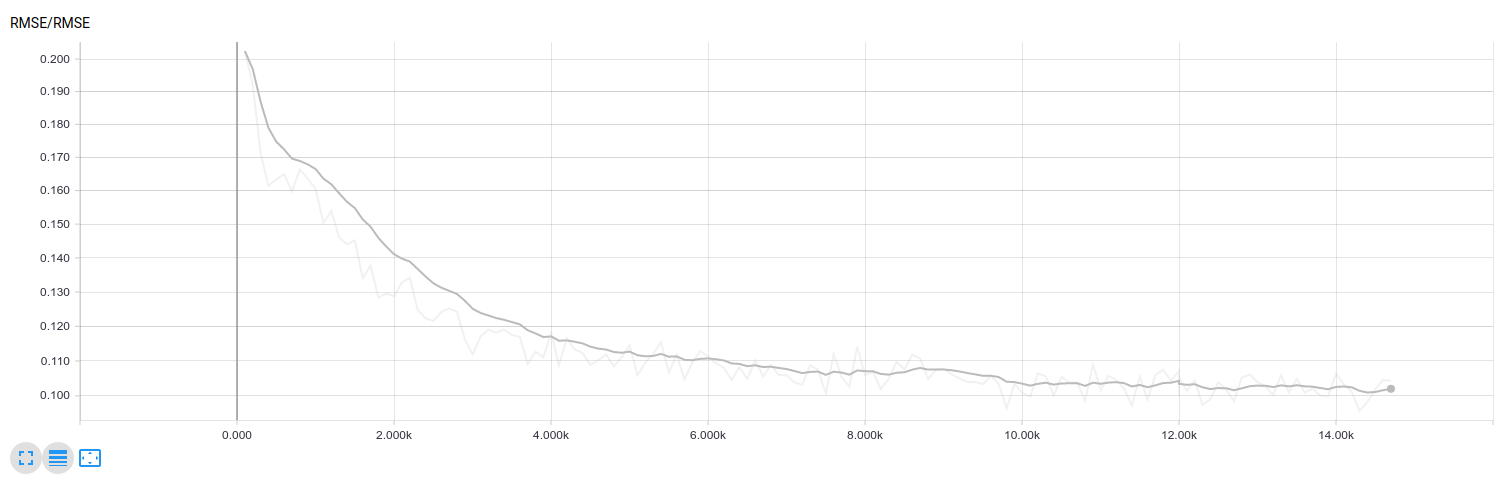
\includegraphics[width=\linewidth]{graphs/B/tycho_1_TRAIN_SELECT_ONE_ADAM_0004_sigmoid.png}
    \caption{Graph of the training error for the duration of the training period}
\end{figure}

\chapter{Tycho1.2 Graphs}


The resultant TensorBoard graph of the training error, from the training of the Tycho1.2 network, from chapter \ref{tycho1.2}.
 
 
\section{Validation}

\begin{figure}[H]
  \centering
    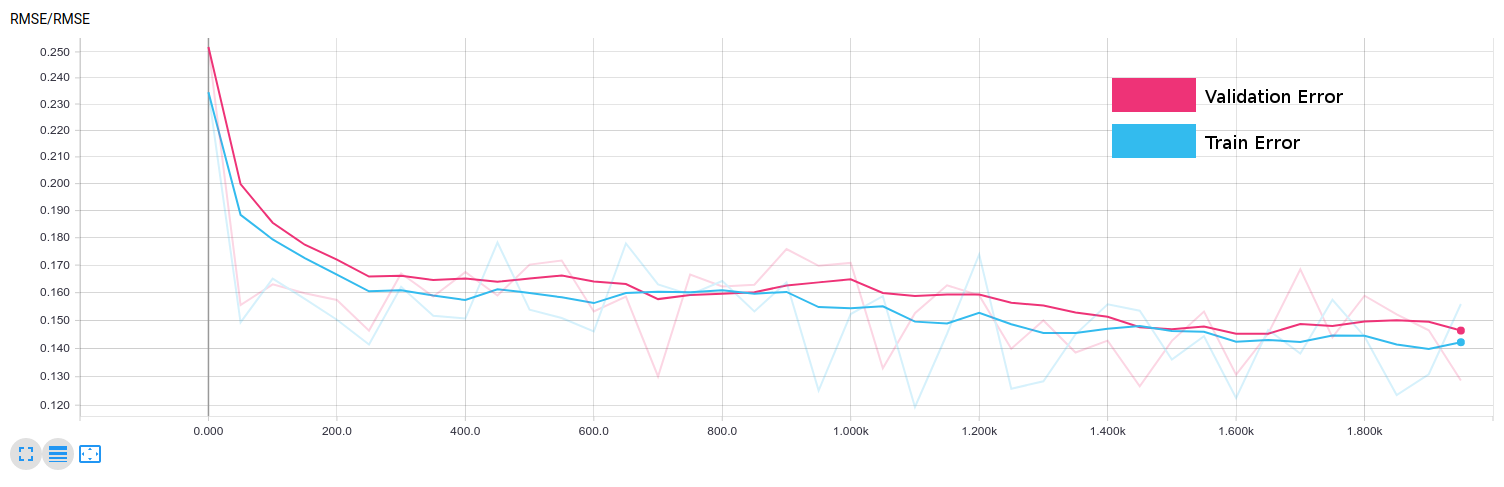
\includegraphics[width=\linewidth]{graphs/C/tycho_1_ADAM_0004_relu.png}
    \caption{Graph of the validation of the Tycho1.2 network.}
\end{figure}

\section{Training}

\begin{figure}[H]
  \centering
    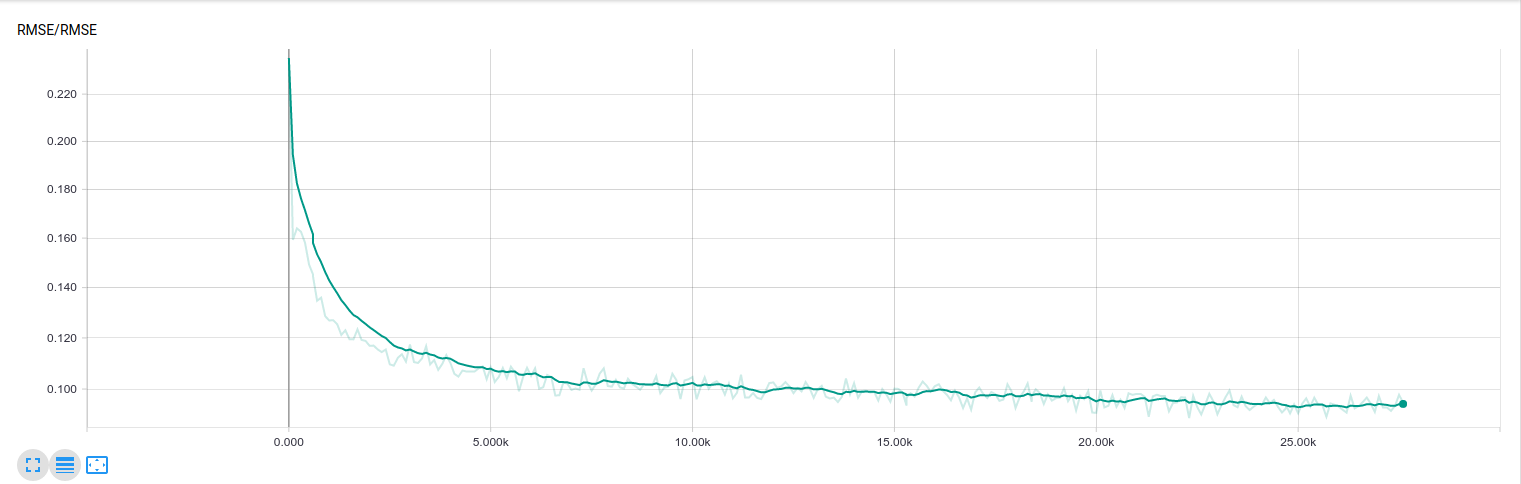
\includegraphics[width=\linewidth]{graphs/C/tycho_12_TRAIN_SELECT_ONE_ADAM_0004_relu.png}
    \caption{Graph of the training error for the duration of the training period}
\end{figure}

\chapter{Tycho2 Graphs}

The resultant TensorBoard graphs of the errors, from the validation, and training (with and without dropout) of the Tycho2 network, from chapter \ref{tycho2}.


\section{Validation}

\begin{figure}[H]
  \centering
    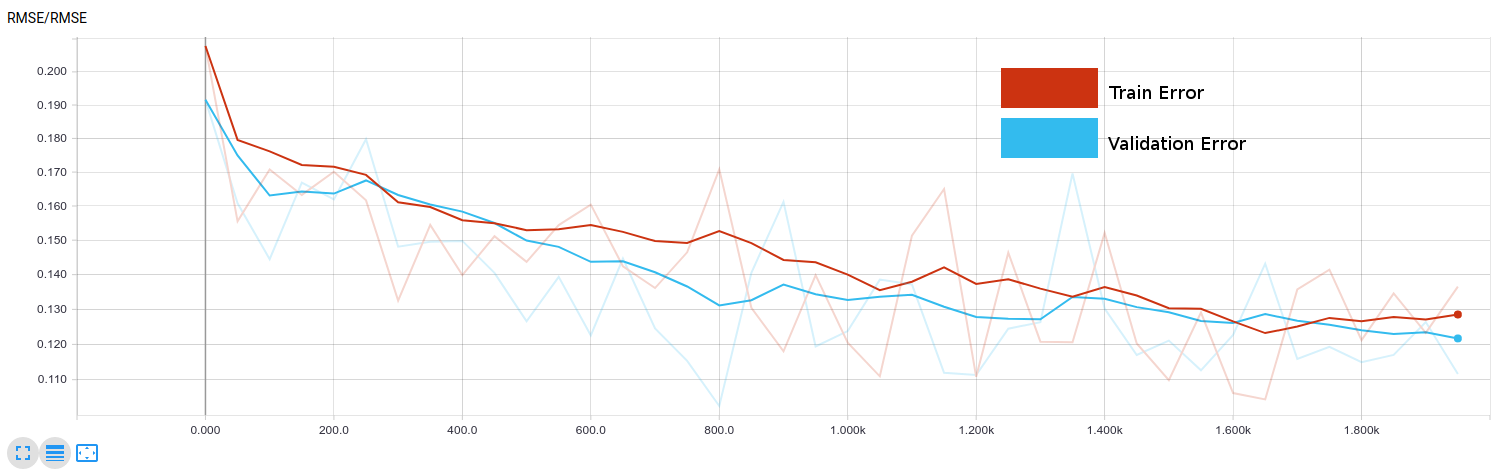
\includegraphics[width=\linewidth]{graphs/D/tycho_2_experiments_ADAM_00004_relu_relu.png}
    \caption{Graph of the validation of the Tycho2 network.}
\end{figure}

\section{Training}
 

\begin{figure}[H]
  \centering
    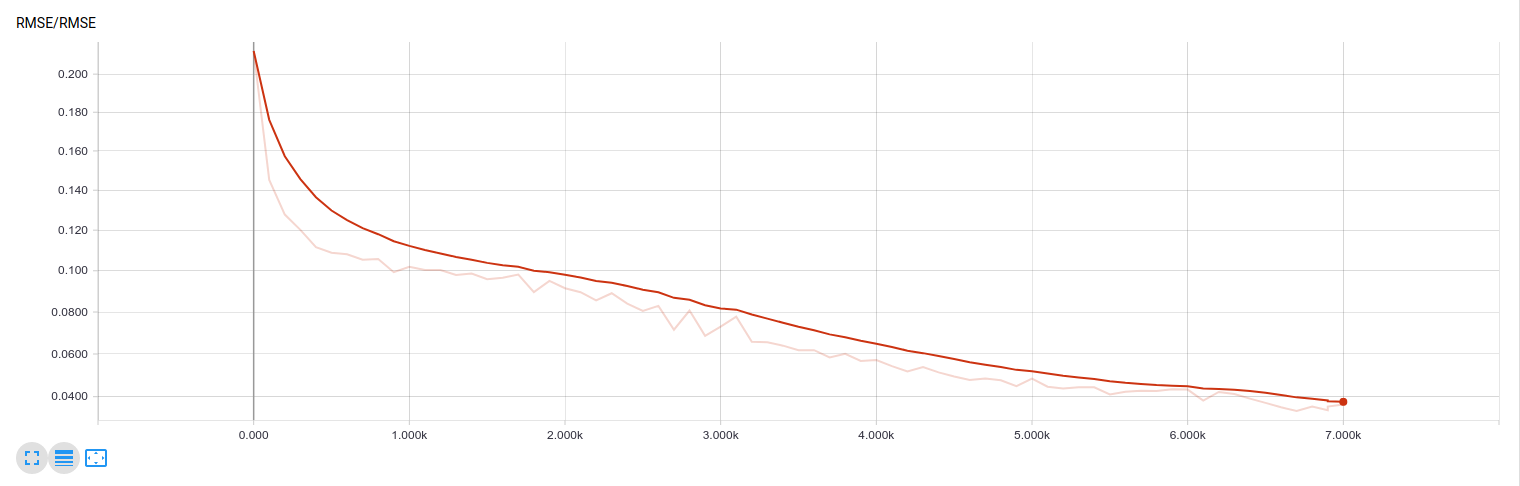
\includegraphics[width=\linewidth]{graphs/D/tycho_2_TRAIN_CONCAT_ADAM_0004_relu_relu_0.png}
    \caption{Graph of the training error for the duration of the training period}
\end{figure}

\section{Training With Dropout}

\begin{figure}[H]
  \centering
    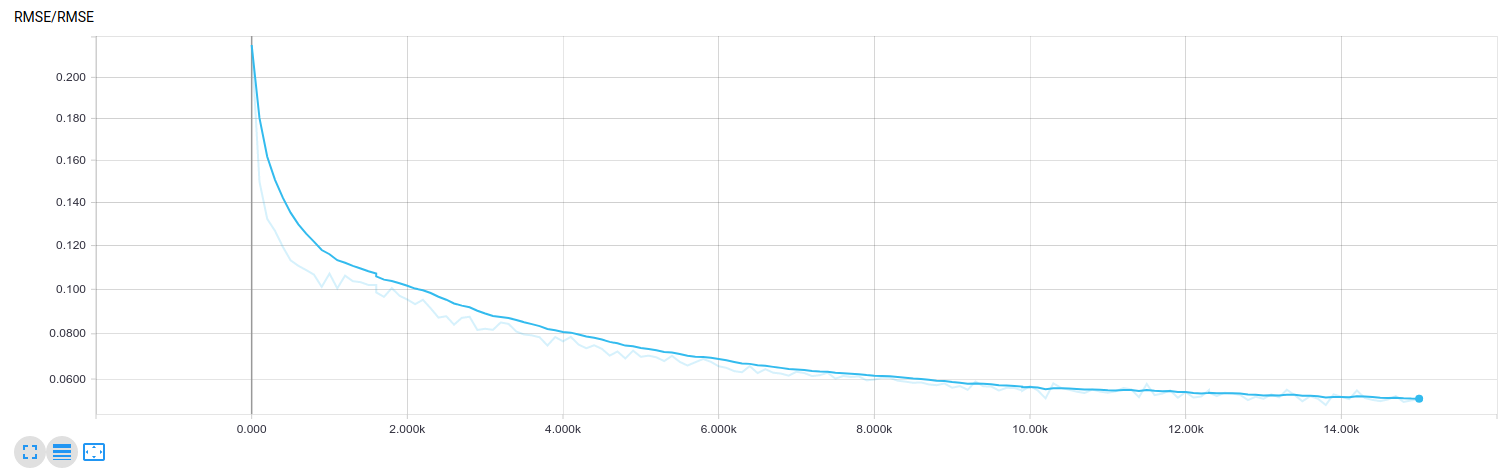
\includegraphics[width=\linewidth]{graphs/D/tycho_2_TRAIN_CONCAT_ADAM_0004_relu_relu_05.png}
    \caption{Graph of the training error for the duration of the training period}
\end{figure}


\chapter{Tycho3 Graphs}

The resultant TensorBoard graphs of the errors, from the validation, and training (with and without dropout) of the Tycho3 network, from chapter \ref{tycho3}.

\section{Validation}

\begin{figure}[H]
  \centering
    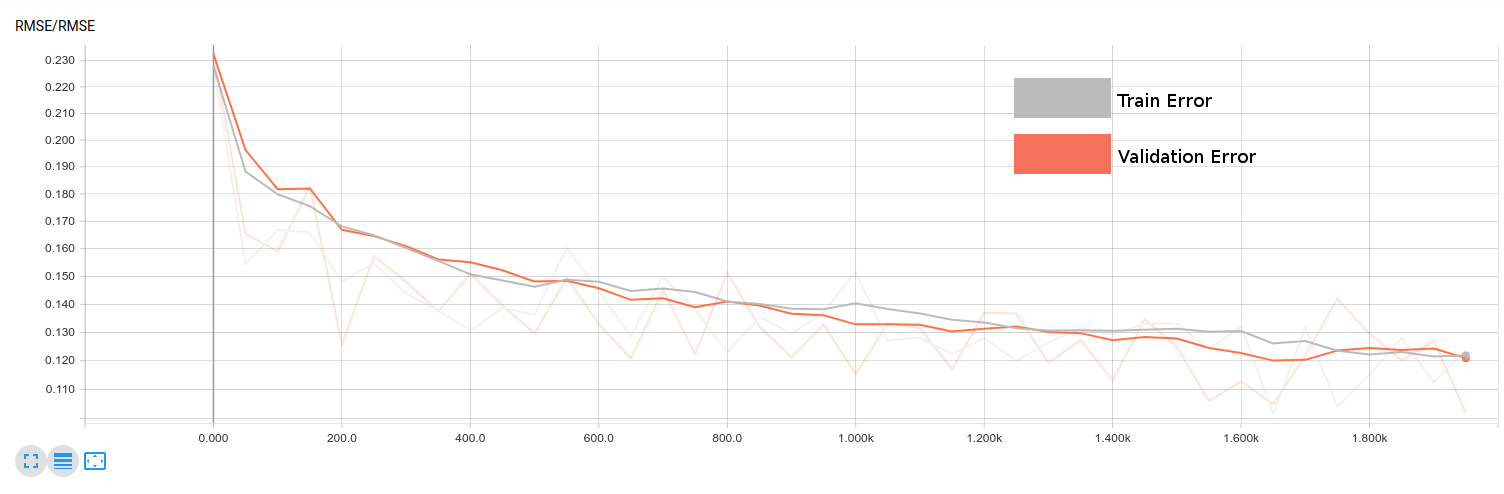
\includegraphics[width=\linewidth]{graphs/E/tycho_2_experiments_ADAM_0004_maxout_relu.png}
    \caption{Graph of the validation of the Tycho3 network.}
\end{figure}

\section{Training}

\begin{figure}[H]
  \centering
    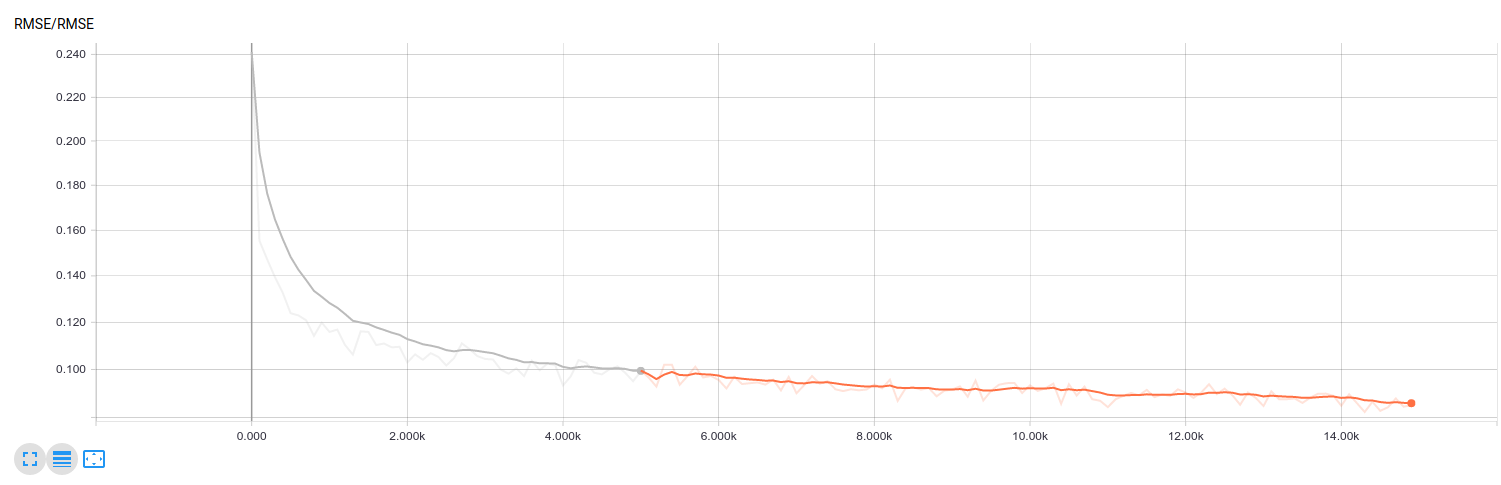
\includegraphics[width=\linewidth]{graphs/E/tycho_21_TRAIN_CONCAT_ADAM_0004_maxout_relu.png}
    \caption{Graph of the training error for the duration of the training period}
\end{figure}

\section{Training With Dropout}

\begin{figure}[H]
  \centering
    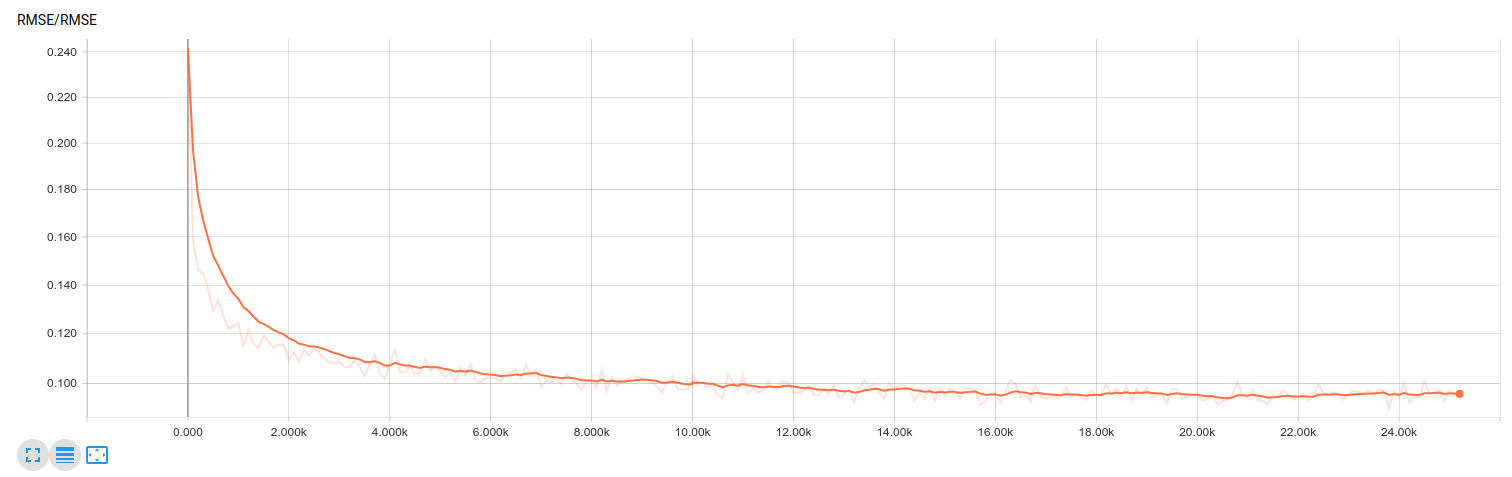
\includegraphics[width=\linewidth]{graphs/E/tycho_21_TRAIN_CONCAT_ADAM_4e-05_maxout_relu_05.png}
    \caption{Graph of the training error for the duration of the training period}
\end{figure}

\chapter{Convolutional Layers Experiment Graphs}

The resultant TensorBoard graphs of the errors, from the varying number of convolutional layers experiment, from chapter \ref{conv-exp}.

\begin{figure}[H]
  \centering
    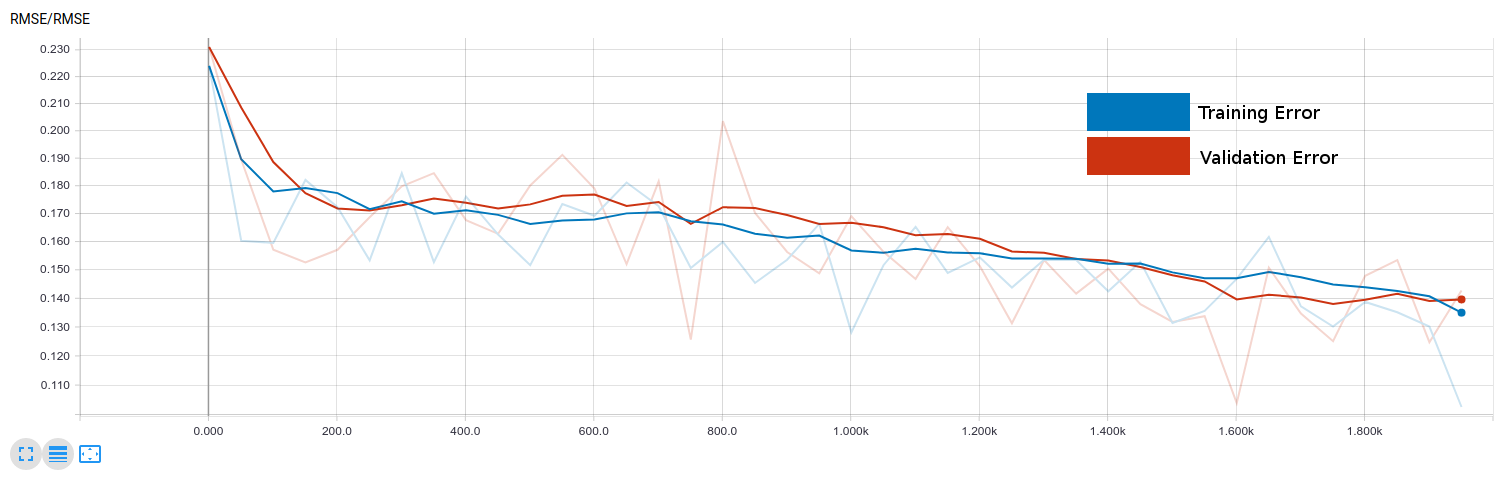
\includegraphics[width=\linewidth]{graphs/F/conv3.png}
    \caption{Graph of experiment results of Tycho1.2 with 3 convolutional layers.}
\end{figure}

\begin{figure}[H]
  \centering
    \includegraphics[width=\linewidth]{graphs/F/conv4.png}
    \caption{Graph of experiment results of Tycho1.2 with 4 convolutional layers.}
\end{figure}


\begin{figure}[H]
  \centering
    \includegraphics[width=\linewidth]{graphs/F/conv5.png}
    \caption{Graph of experiment results of Tycho1.2 with 5 convolutional layers.}
\end{figure}



\chapter{Email Exchange With Sander Dieleman}

The response to the email sent by the student to Sander Dieleman.

\begin{figure}[H]
  \centering
    \includegraphics[width=\linewidth]{graphs/G/email.png}
    \caption{Email exchange with Sander Dieleman in regards to the maxout layer configuration in his solution}
    \label{email}
\end{figure}



\renewcommand{\bibname}{References}
\bibliographystyle{unsrt}
\bibliography{references}

\end{document}

